\pagestyle{hedra}
\label{hedra}

%\begin{textblock*}{5.625in}(0pt,0pt)%
%\vspace*{-3.5cm}
%\hspace*{-2.77cm}\includegraphics*[width=175.2mm]{./propagandas/HEDRA.pdf}
%\end{textblock*}

%\pagebreak

\begin{center}
\hspace*{-3.6cm}\raisebox{5cm}{\rotatebox[origin=t]{90}{\huge\textbf{Lançamento}}}
\hspace*{3.1cm}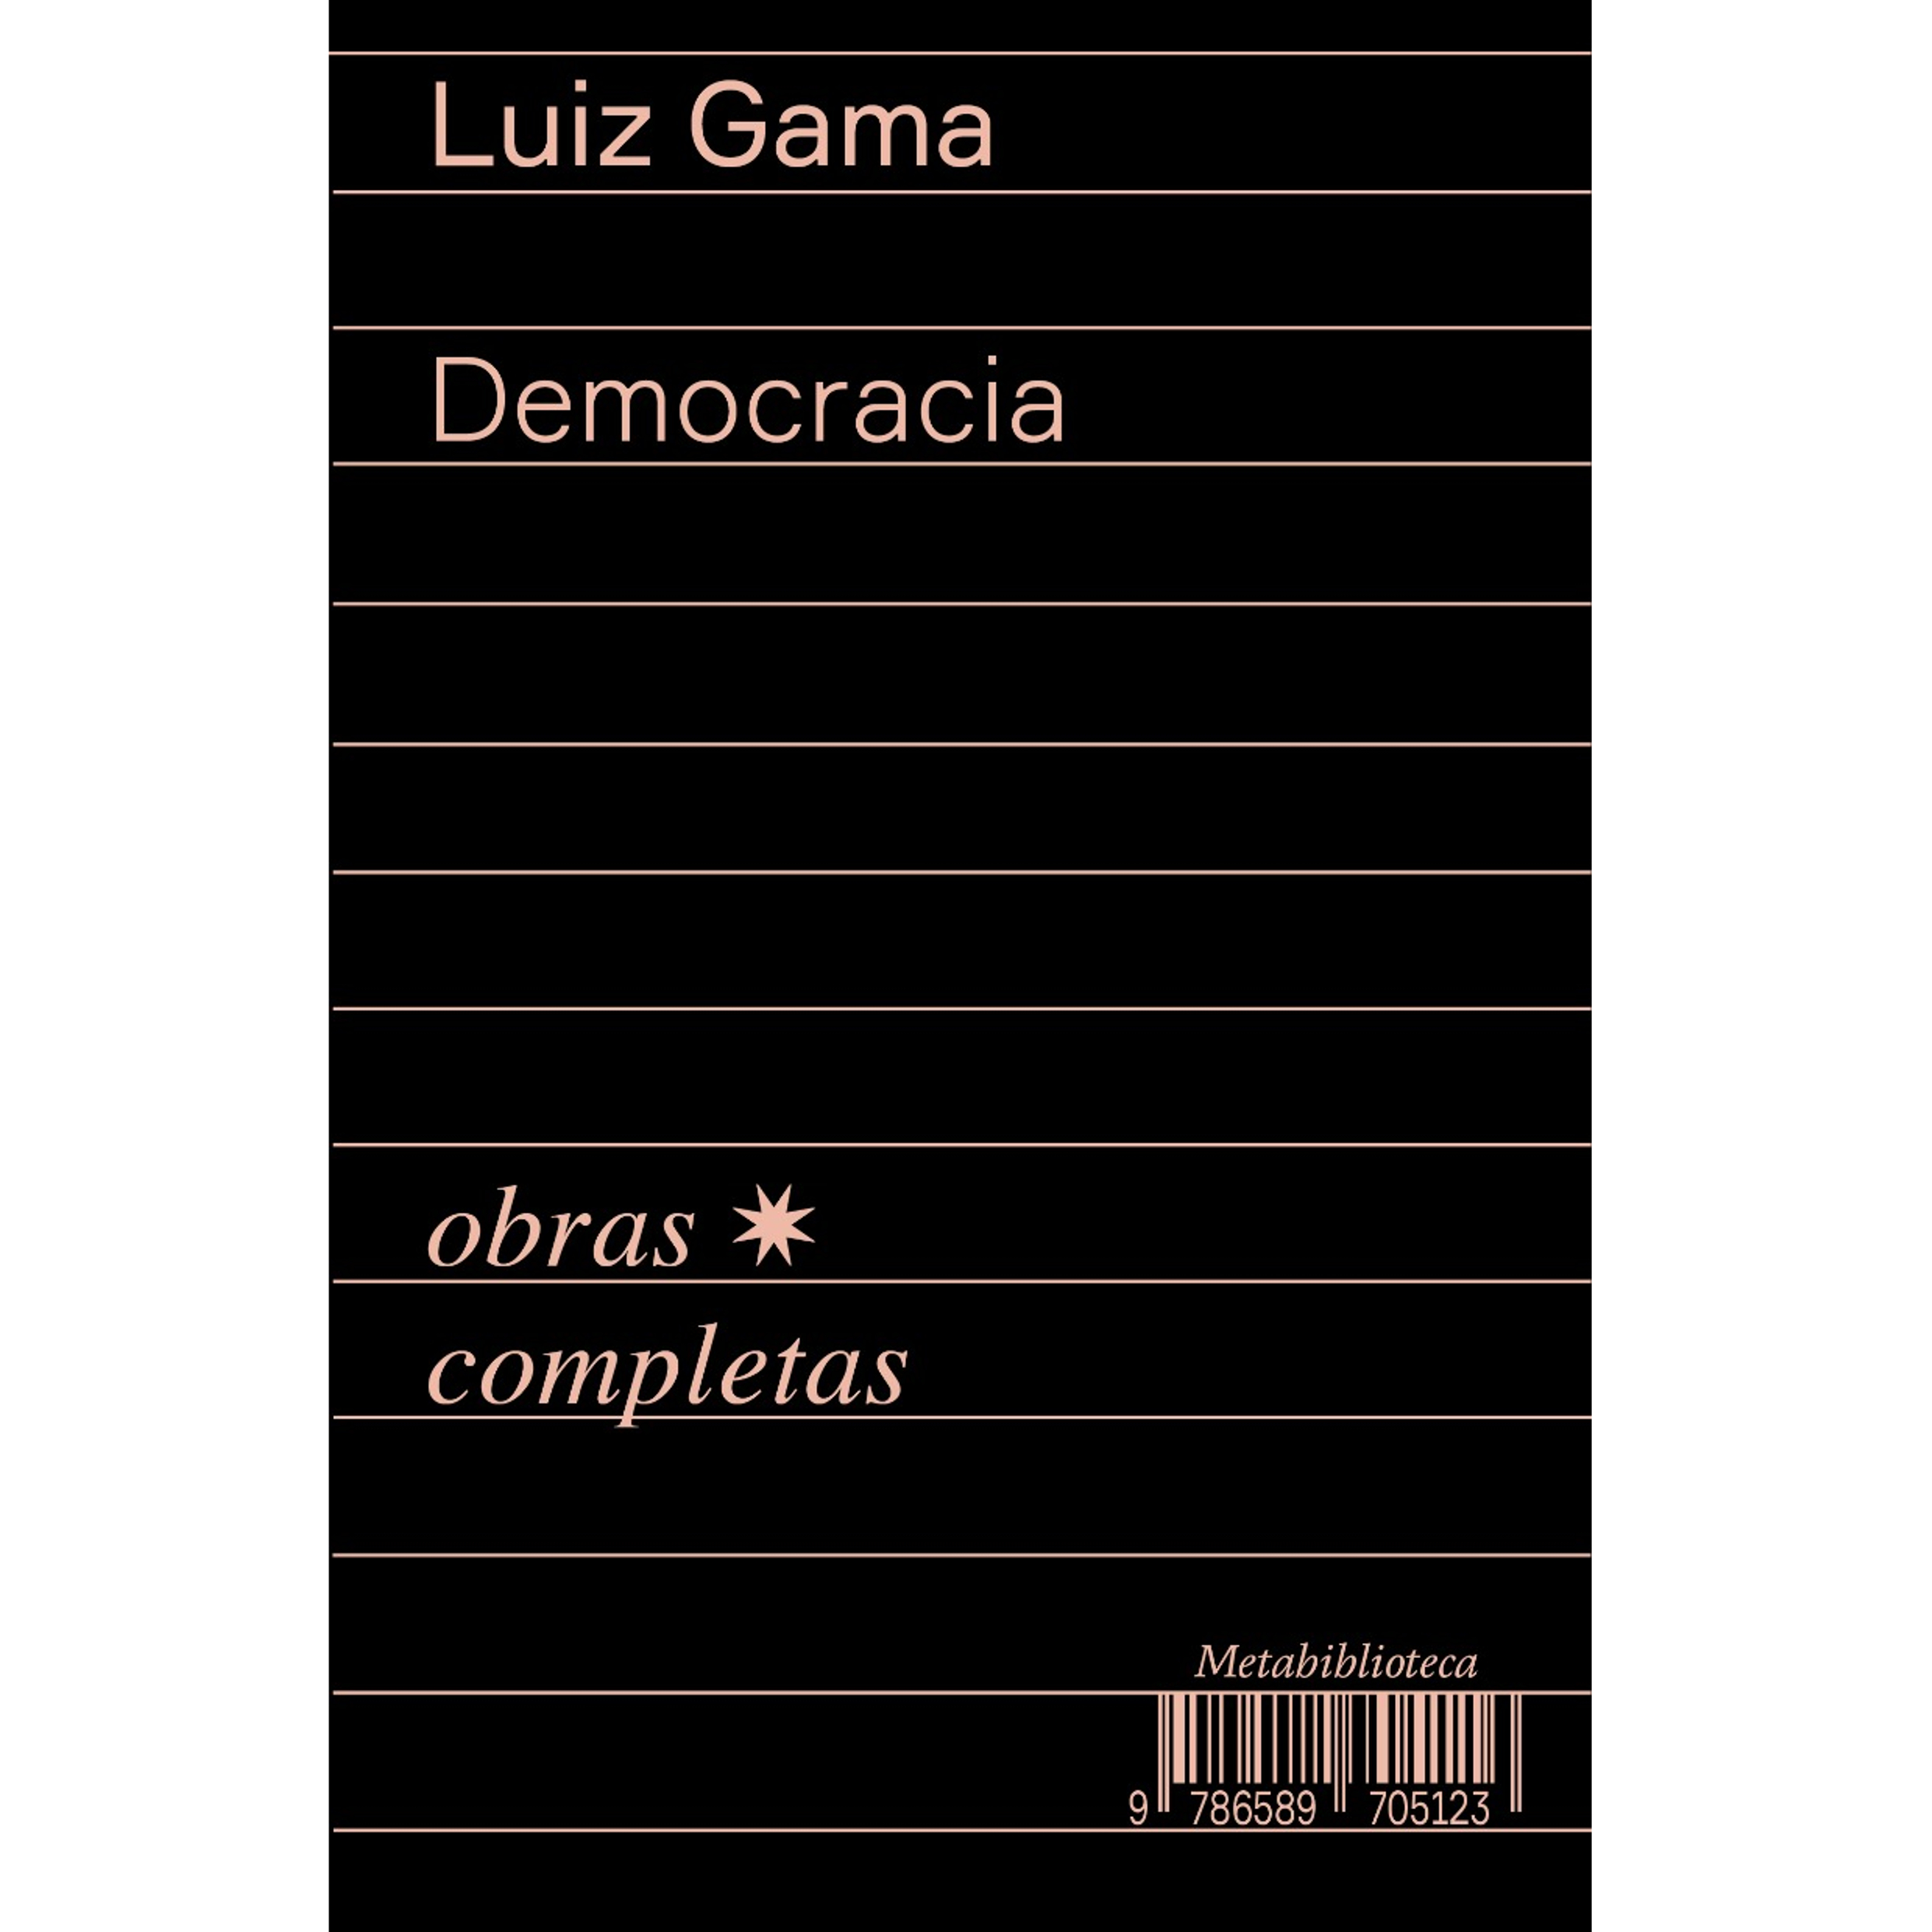
\includegraphics[width=74mm]{./grid/democracia.jpg}
\end{center}

\hspace*{-7cm}\hrulefill\hspace*{-7cm}

\medskip

\noindent{}\textit{Democracia} integra as \textit{Obras completas} de Luiz Gama, advogado negro e abolicionista, a serem lançadas em 11 volumes com cerca de 800 escritos --- 600 inéditos ---, revelando as diversas facetas e estilos empregados pelo escritor para advogar pela grande causa de sua vida: a abolição da escravidão e a emancipação negra. Esquecidos em parte por quase dois séculos, os textos foram recuperados pelo pesquisador Bruno Rodrigues de Lima, que passou nove anos localizando-os em arquivos da imprensa e do judiciário de todo o país.

Os textos e artigos incluídos em \textit{Democracia} foram publicados originalmente entre os anos de 1866 e 1869. Nesses artigos, Luiz Gama se manifesta publicamente sobre educação, política e direitos universais. \hlc{Lançando mão de uma estratégia autoral ousada, que incluía o uso de pseudônimos, Gama defende abertamente o direito à educação universal e as obrigações do Estado em garantir um ensino público de qualidade} em todos os níveis como os fundamentos da vida democrática.

\vfill

\noindent\begin{minipage}[c]{1\linewidth}
{\small\textbf{
\hspace*{-.1cm}Editora: Hedra\\
Título: Democracia (1866--1869)\\
Autor: Luiz Gama\\ 
ISBN: 978-65-89705-12-3\\
Páginas: 506\\
Formato: 13,3x21\,cm\\
Preço: R\$ 110,00\\
}}
\end{minipage}

\pagebreak

\begin{center}
\hspace*{.5cm}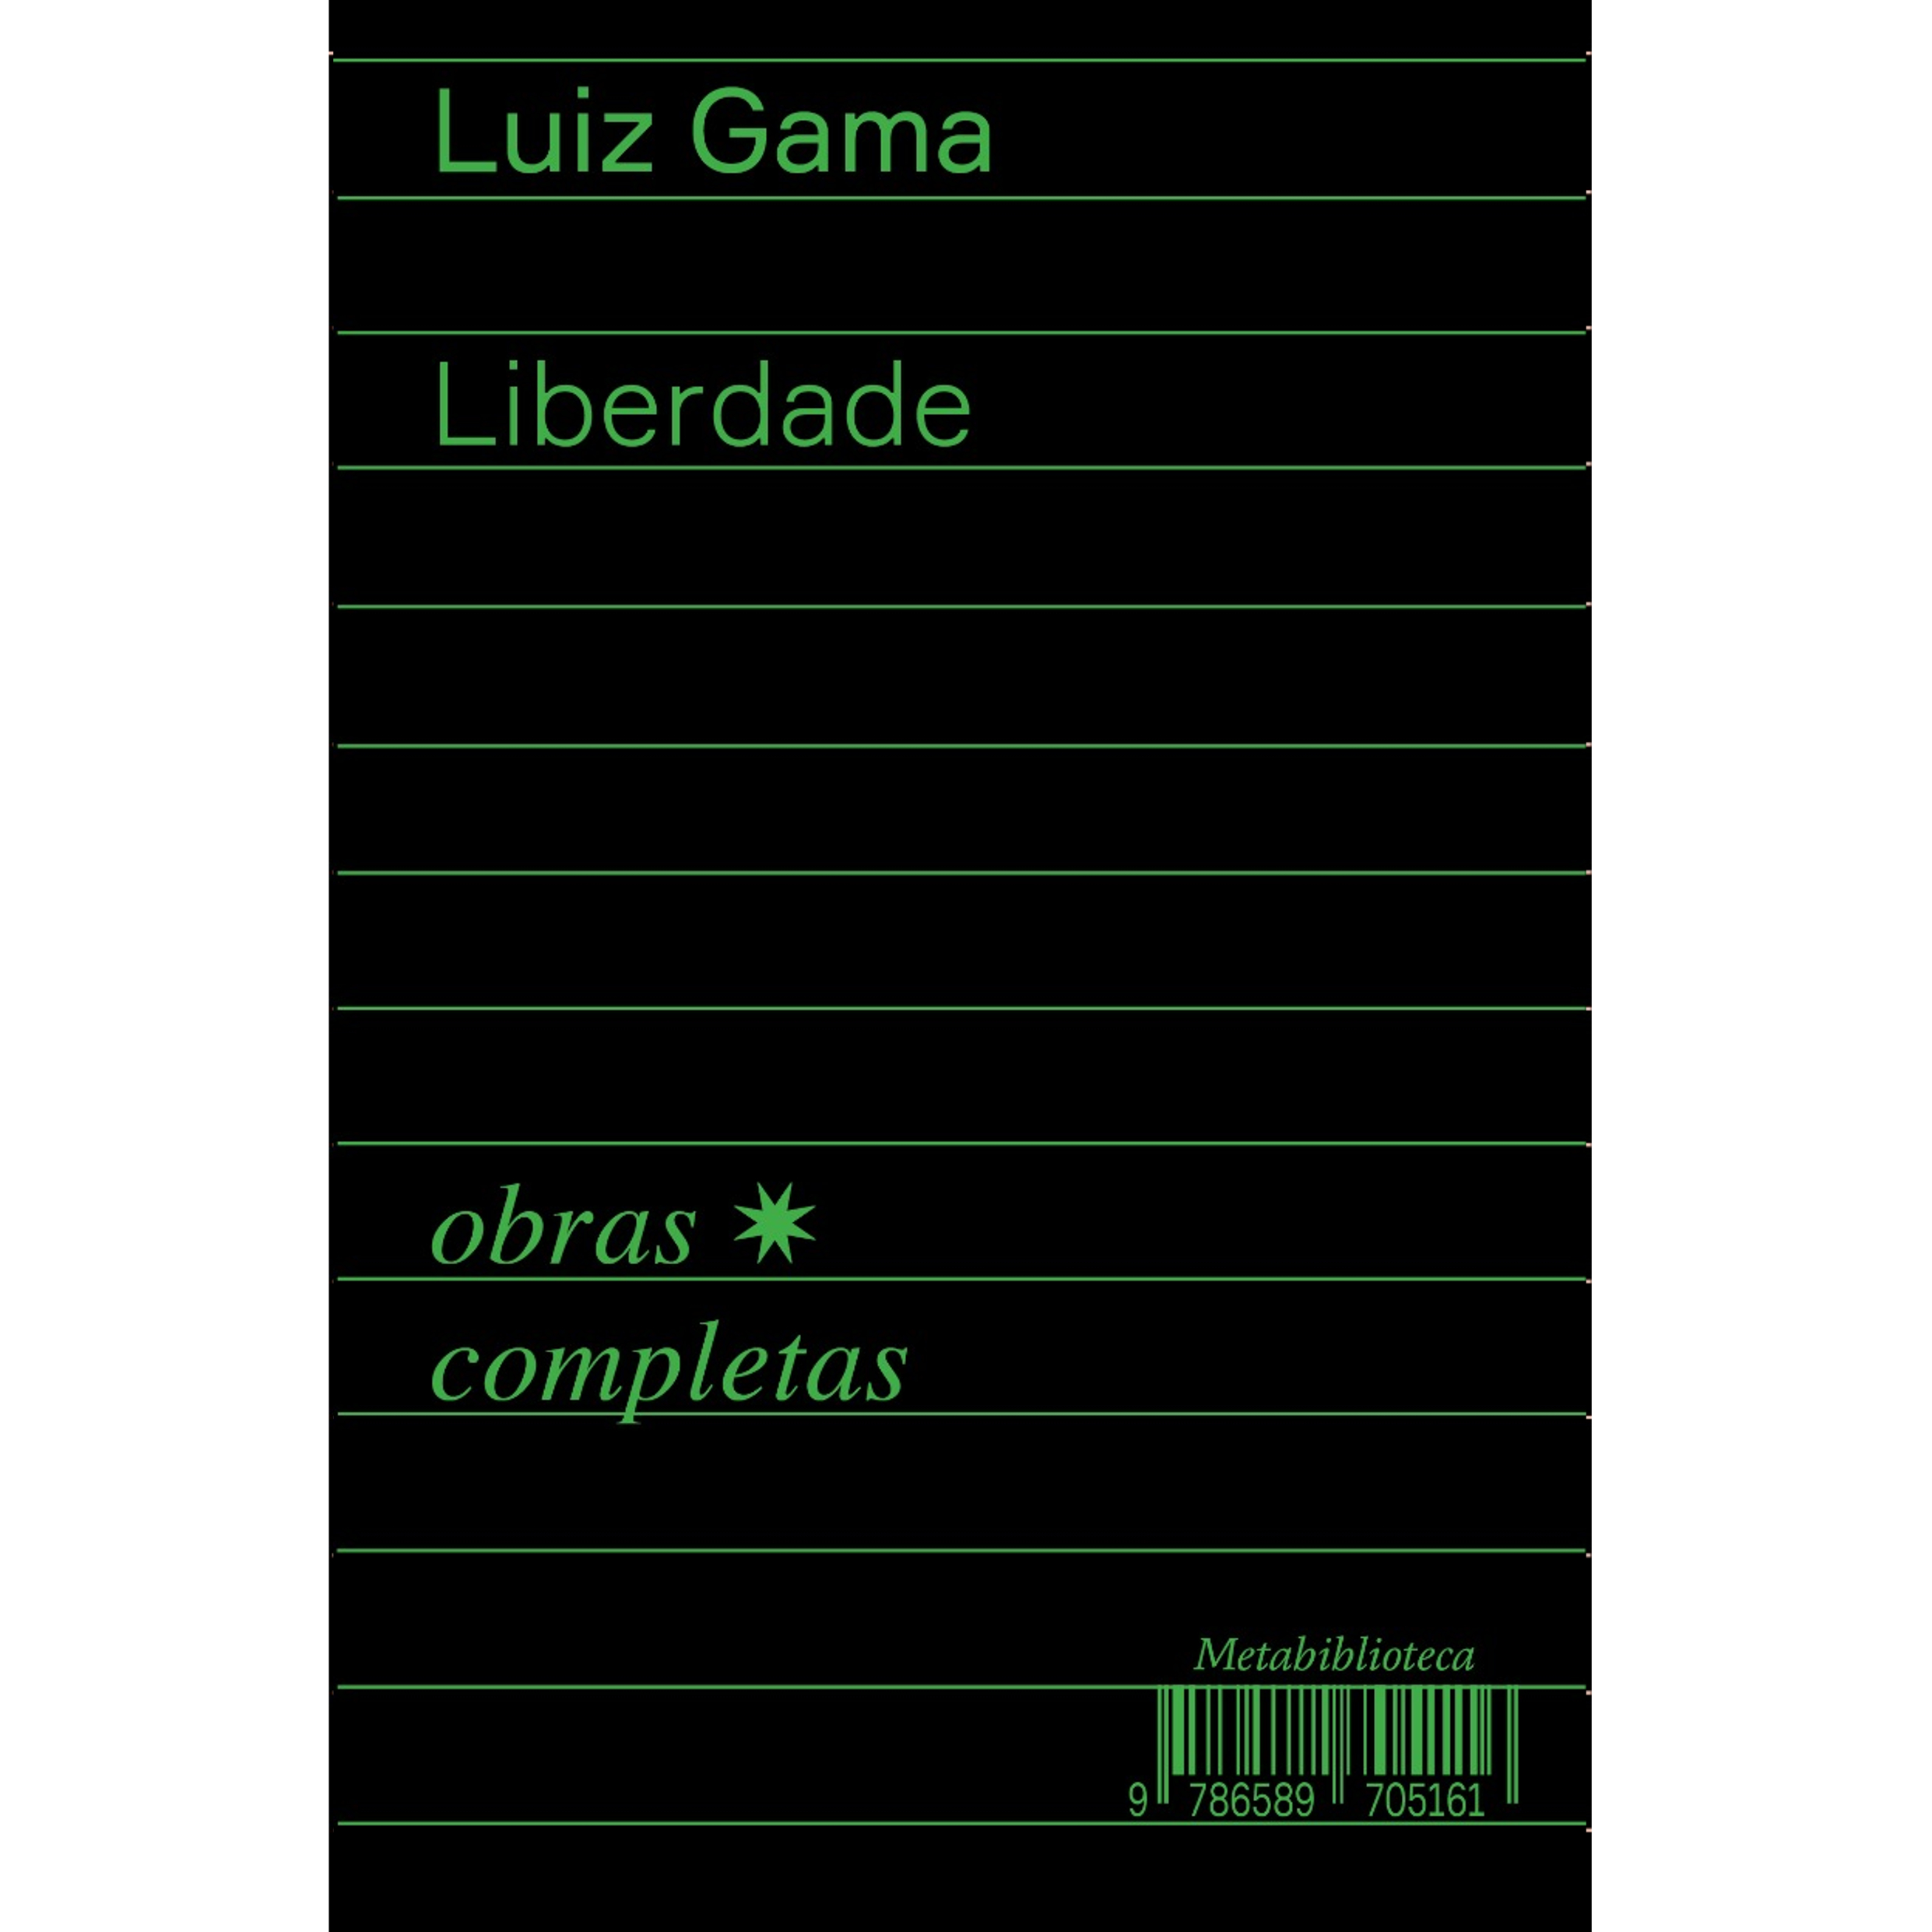
\includegraphics[width=74mm]{./grid/liberdade.jpg}
\end{center}

\hspace*{-7cm}\hrulefill\hspace*{-7cm}

\medskip

\noindent{}\textit{Liberdade} integra as \textit{Obras completas} de Luiz Gama, advogado negro e abolicionista, a serem lançadas em 11 volumes com cerca de 800 escritos --- 600 inéditos ---, revelando as diversas facetas e estilos empregados pelo escritor para advogar pela grande causa de sua vida: a abolição da escravidão e a emancipação negra. Esquecidos em parte por quase dois séculos, os textos foram recuperados pelo pesquisador Bruno Rodrigues de Lima, que passou nove anos localizando-os em arquivos da imprensa e do judiciário de todo o país.

\hlc{Os textos deste volume são fruto da campanha pela abolição radical, que também visava à garantia da educação e cidadania para os libertos: o abolicionismo de Gama exigia cidadania e igualdade de fato e de direito}. O advogado também refletia sobre o processo histórico em curso, e propunha soluções políticas para o tempo presente, revelando sua natureza intelectual até hoje pouco conhecida e quase sempre não reconhecida.

\vfill

\noindent\begin{minipage}[c]{.5\linewidth}
{\small\textbf{
\hspace*{-.1cm}Editora: Hedra\\
Título: Liberdade (1880--1882)\\
Autor: Luiz Gama\\ 
ISBN: 978-65-89705-16-1\\
Páginas: 446\\
Formato: 13,3x21\,cm\\
Preço: R\$ 99,90\\
}}
\end{minipage}

\pagebreak

\begin{center}
\hspace*{-3.6cm}\raisebox{5cm}{\rotatebox[origin=t]{90}{\huge\textbf{Lançamento}}}
\hspace*{3.1cm}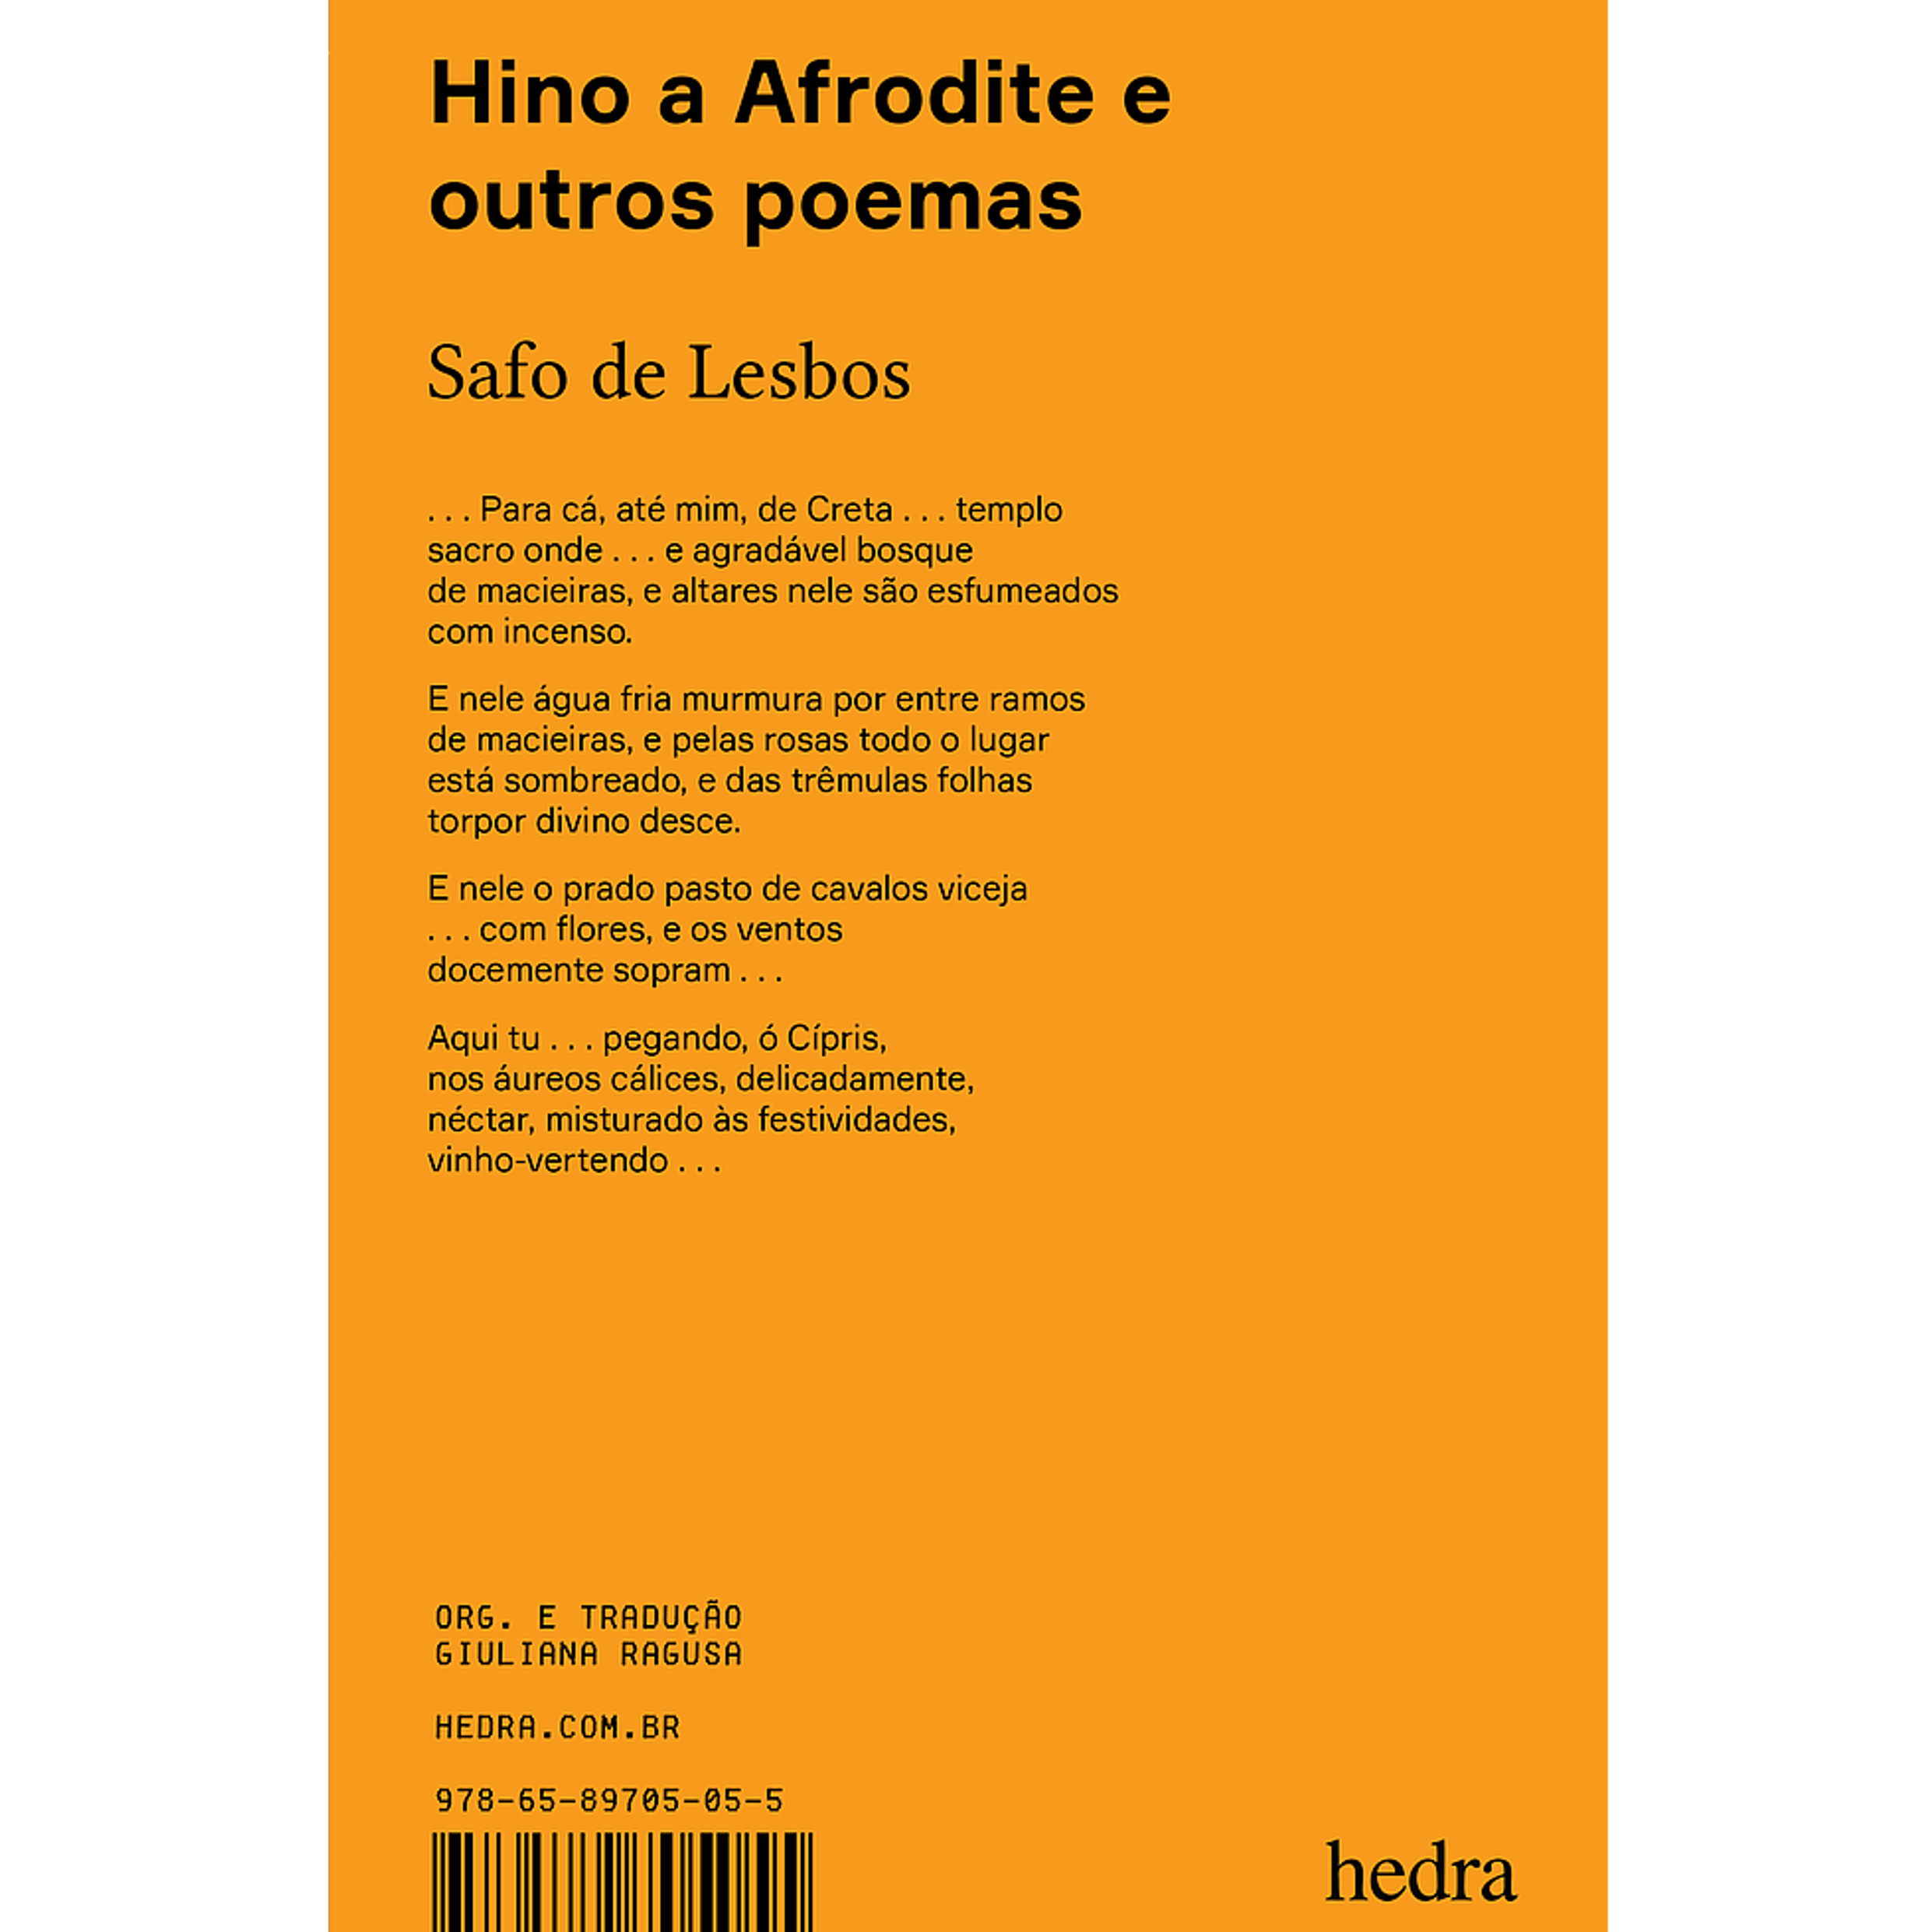
\includegraphics[width=74mm]{./grid/safo.jpg}
\end{center}

\hspace*{-7cm}\hrulefill\hspace*{-7cm}

\medskip

\noindent{}Reunião de \hlc{textos remanescentes da mélica de Safo, ou seja, as canções para performance ao som da lira. Os textos aqui são traduzidos e anotados por Giuliana Ragusa em segunda edição --- com novos poemas, atualizações e em versão bilíngue} ---, autora que ganhou o Jabuti 2006 com um livro sobre a lírica da poeta, a única mulher entre os grandes da época. Para esta edição foram selecionados a única canção completa e os fragmentos mais legíveis de canções do corpus de Safo. As anotações de leitura buscam lançar luz sobre elementos relevantes da estrutura, conteúdo ou transmissão dos fragmentos organizados tematicamente. Precede a tradução anotada uma introdução sobre a poeta, sua poesia e o contexto em que se produziu e circulou, o gênero mélico, a fortuna crítica sobre ela, a transmissão de sua obra, e as outras poetas mulheres de que se tem notícia.

\vfill

\noindent\begin{minipage}[c]{1\linewidth}
{\small\textbf{
\hspace*{-.1cm}Editora: Hedra\\
Título: Hino a Afrodite e outros poemas\\
Autor: Safo de Lesbos\\ 
ISBN: 978-65-89705-05-5\\
Páginas: 212\\
Formato: 13,3x21\,cm\\
Preço: R\$ 69,00\\
}}
\end{minipage}

\pagebreak

\begin{center}
\hspace*{.5cm}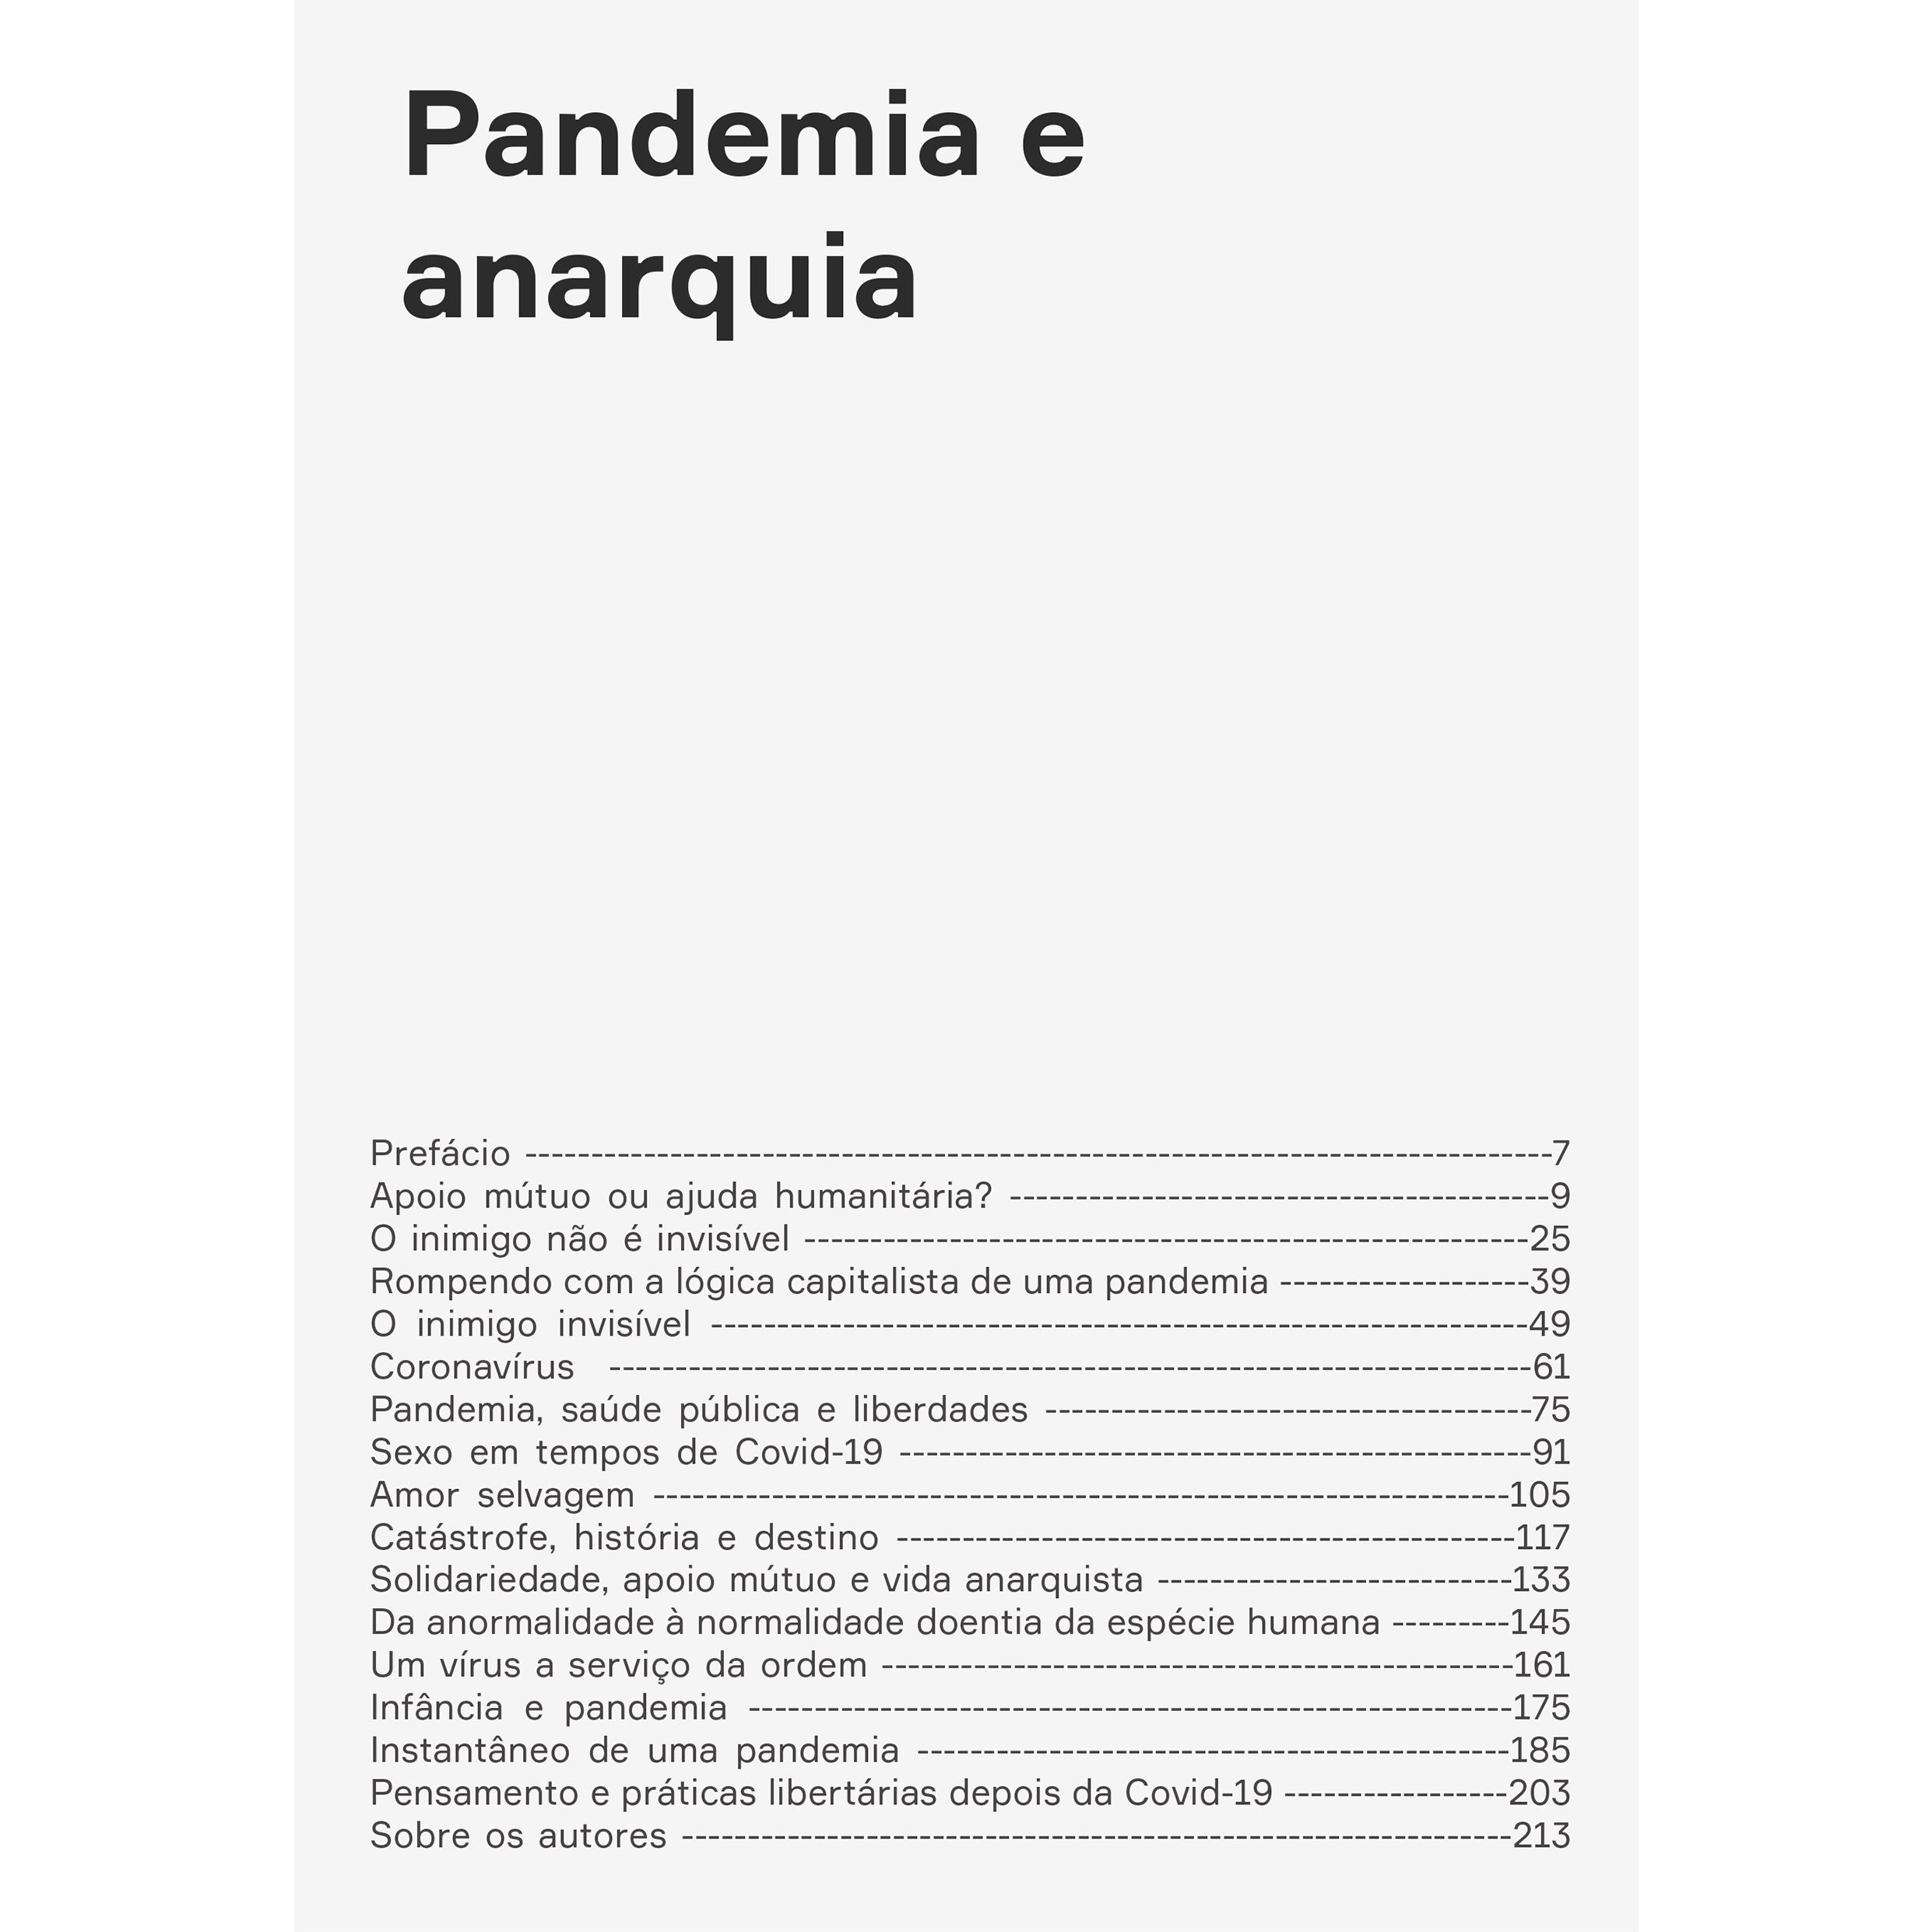
\includegraphics[width=74mm]{./grid/pandemia.jpg}
\end{center}

\hspace*{-7cm}\hrulefill\hspace*{-7cm}

\medskip

\noindent{}\textit{Pandemia e anarquia} reúne quinze ensaios de pesquisadores das práticas libertárias que analisam as implicações sociopolíticas do novo coronavírus e sua relação com os modos de existência. Além da Somaterapia e de pesquisadores do Nu-Sol (Núcleo de Sociabilidade Libertária), este livro traz escritos de historiadores e cientistas políticos residentes em diversos espaços do planeta. \hlc{Perpassando diversas esferas das relações humanas, da economia e da ciência às relações amorosas e ao ser criança durante a pandemia, os escritos insurgem-se contra a suposta ruptura com o mundo dado antes da Covid-19 para analisar e estancar a racionalidade neoliberal, e a chamada crise sanitária}. Com isso, traçam a afirmação de uma vida outra no presente.


\vfill

\noindent\begin{minipage}[c]{.5\linewidth}
{\small\textbf{
\hspace*{-.1cm}Editora: Hedra\\
Título: Pandemia e anarquia\\
Autor: Edson Passetti, João da Mata e José Maria Carvalho Ferreira (orgs.)\\ 
ISBN: 978-65-89705-04-8\\
Páginas: 220\\
Formato: 16x23\,cm\\
Preço: R\$ 69,00\\
}}
\end{minipage}

\pagebreak

\begin{center}
\hspace*{-3.6cm}\raisebox{5cm}{\rotatebox[origin=t]{90}{\huge\textbf{Lançamento}}}
\hspace*{3.1cm}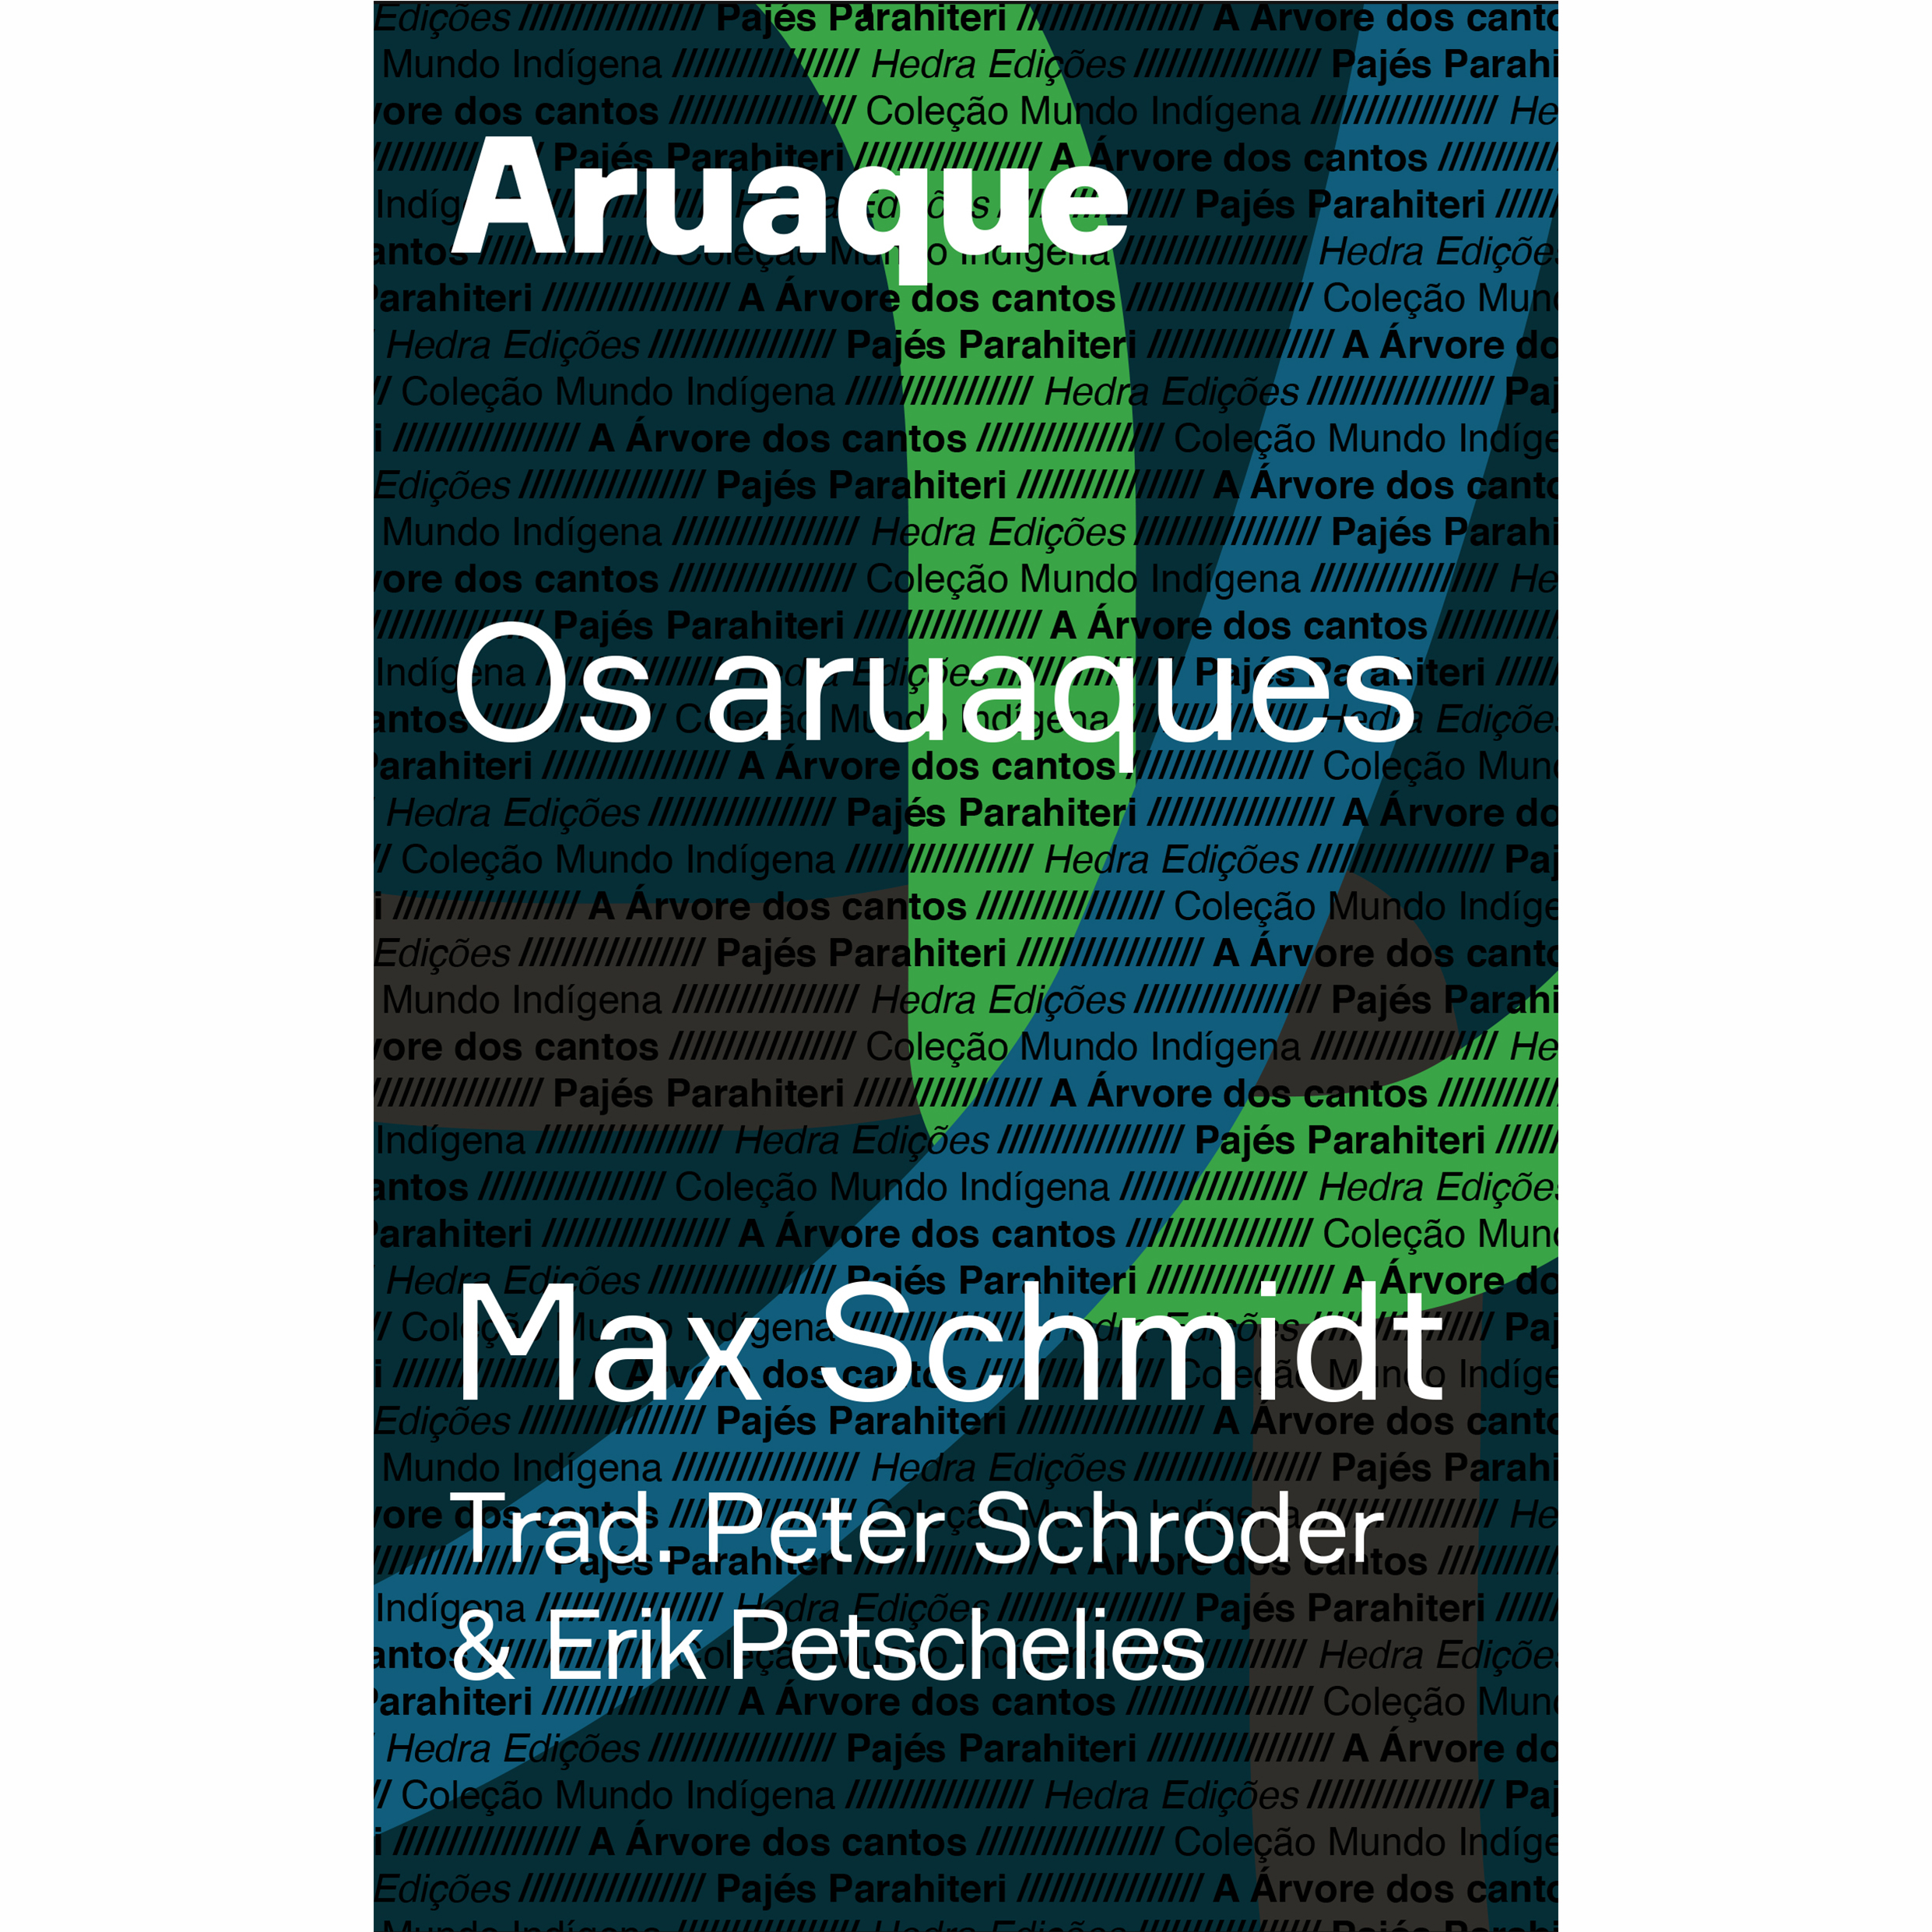
\includegraphics[width=74mm]{./grid/aruaque.jpg}
\end{center}

\hspace*{-7cm}\hrulefill\hspace*{-7cm}

\medskip

\noindent{}\textit{Os aruaques} é um \hlc{livro clássico, escrito antes da Primeira Guerra Mundial, sobre os povos indígenas falantes de línguas aruaque. Durante suas expedições, Max Schmidt já tinha observado a influência cultural dos povos aruaques sobre grupos diferenciados, o que estimulou o interesse por sua enorme expansão geográfica nas terras baixas da América do Sul: o problema central não seria descobrir a origem geográfica dos aruaques, mas explicar sua dinâmica cultural}. Schmidt opera com distinções claras entre fenômenos como língua e cultura e conceitos como aculturação, difusão e mudança cultural em termos gerais. Seu argumento principal é que outros autores, anteriores a ele, não teriam levantado as questões certas sobre a expansão dos aruaques, por isso a falta de respostas satisfatórias. Sua teoria de fato é diferente dos antecessores, mostrando grande originalidade para a época. \textit{Die Aruaken} é a segunda tese de doutorado de Max Schmidt (1874--1950), que já tinha realizado três expedições científicas na América do Sul, em 1900--01, 1910 e 1914.

\vfill

\noindent\begin{minipage}[c]{1\linewidth}
{\small\textbf{
\hspace*{-.1cm}Editora: Hedra\\
Título: Os Aruaques\\
Autor: Max Schmidt\\ 
ISBN: 978-65-89705-22-2\\
Páginas: 192 (provisório)\\
Formato: 13,3x21\,cm\\
Preço: R\$ 59,90\\
}}
\end{minipage}

\pagebreak

\begin{center}
\hspace*{.5cm}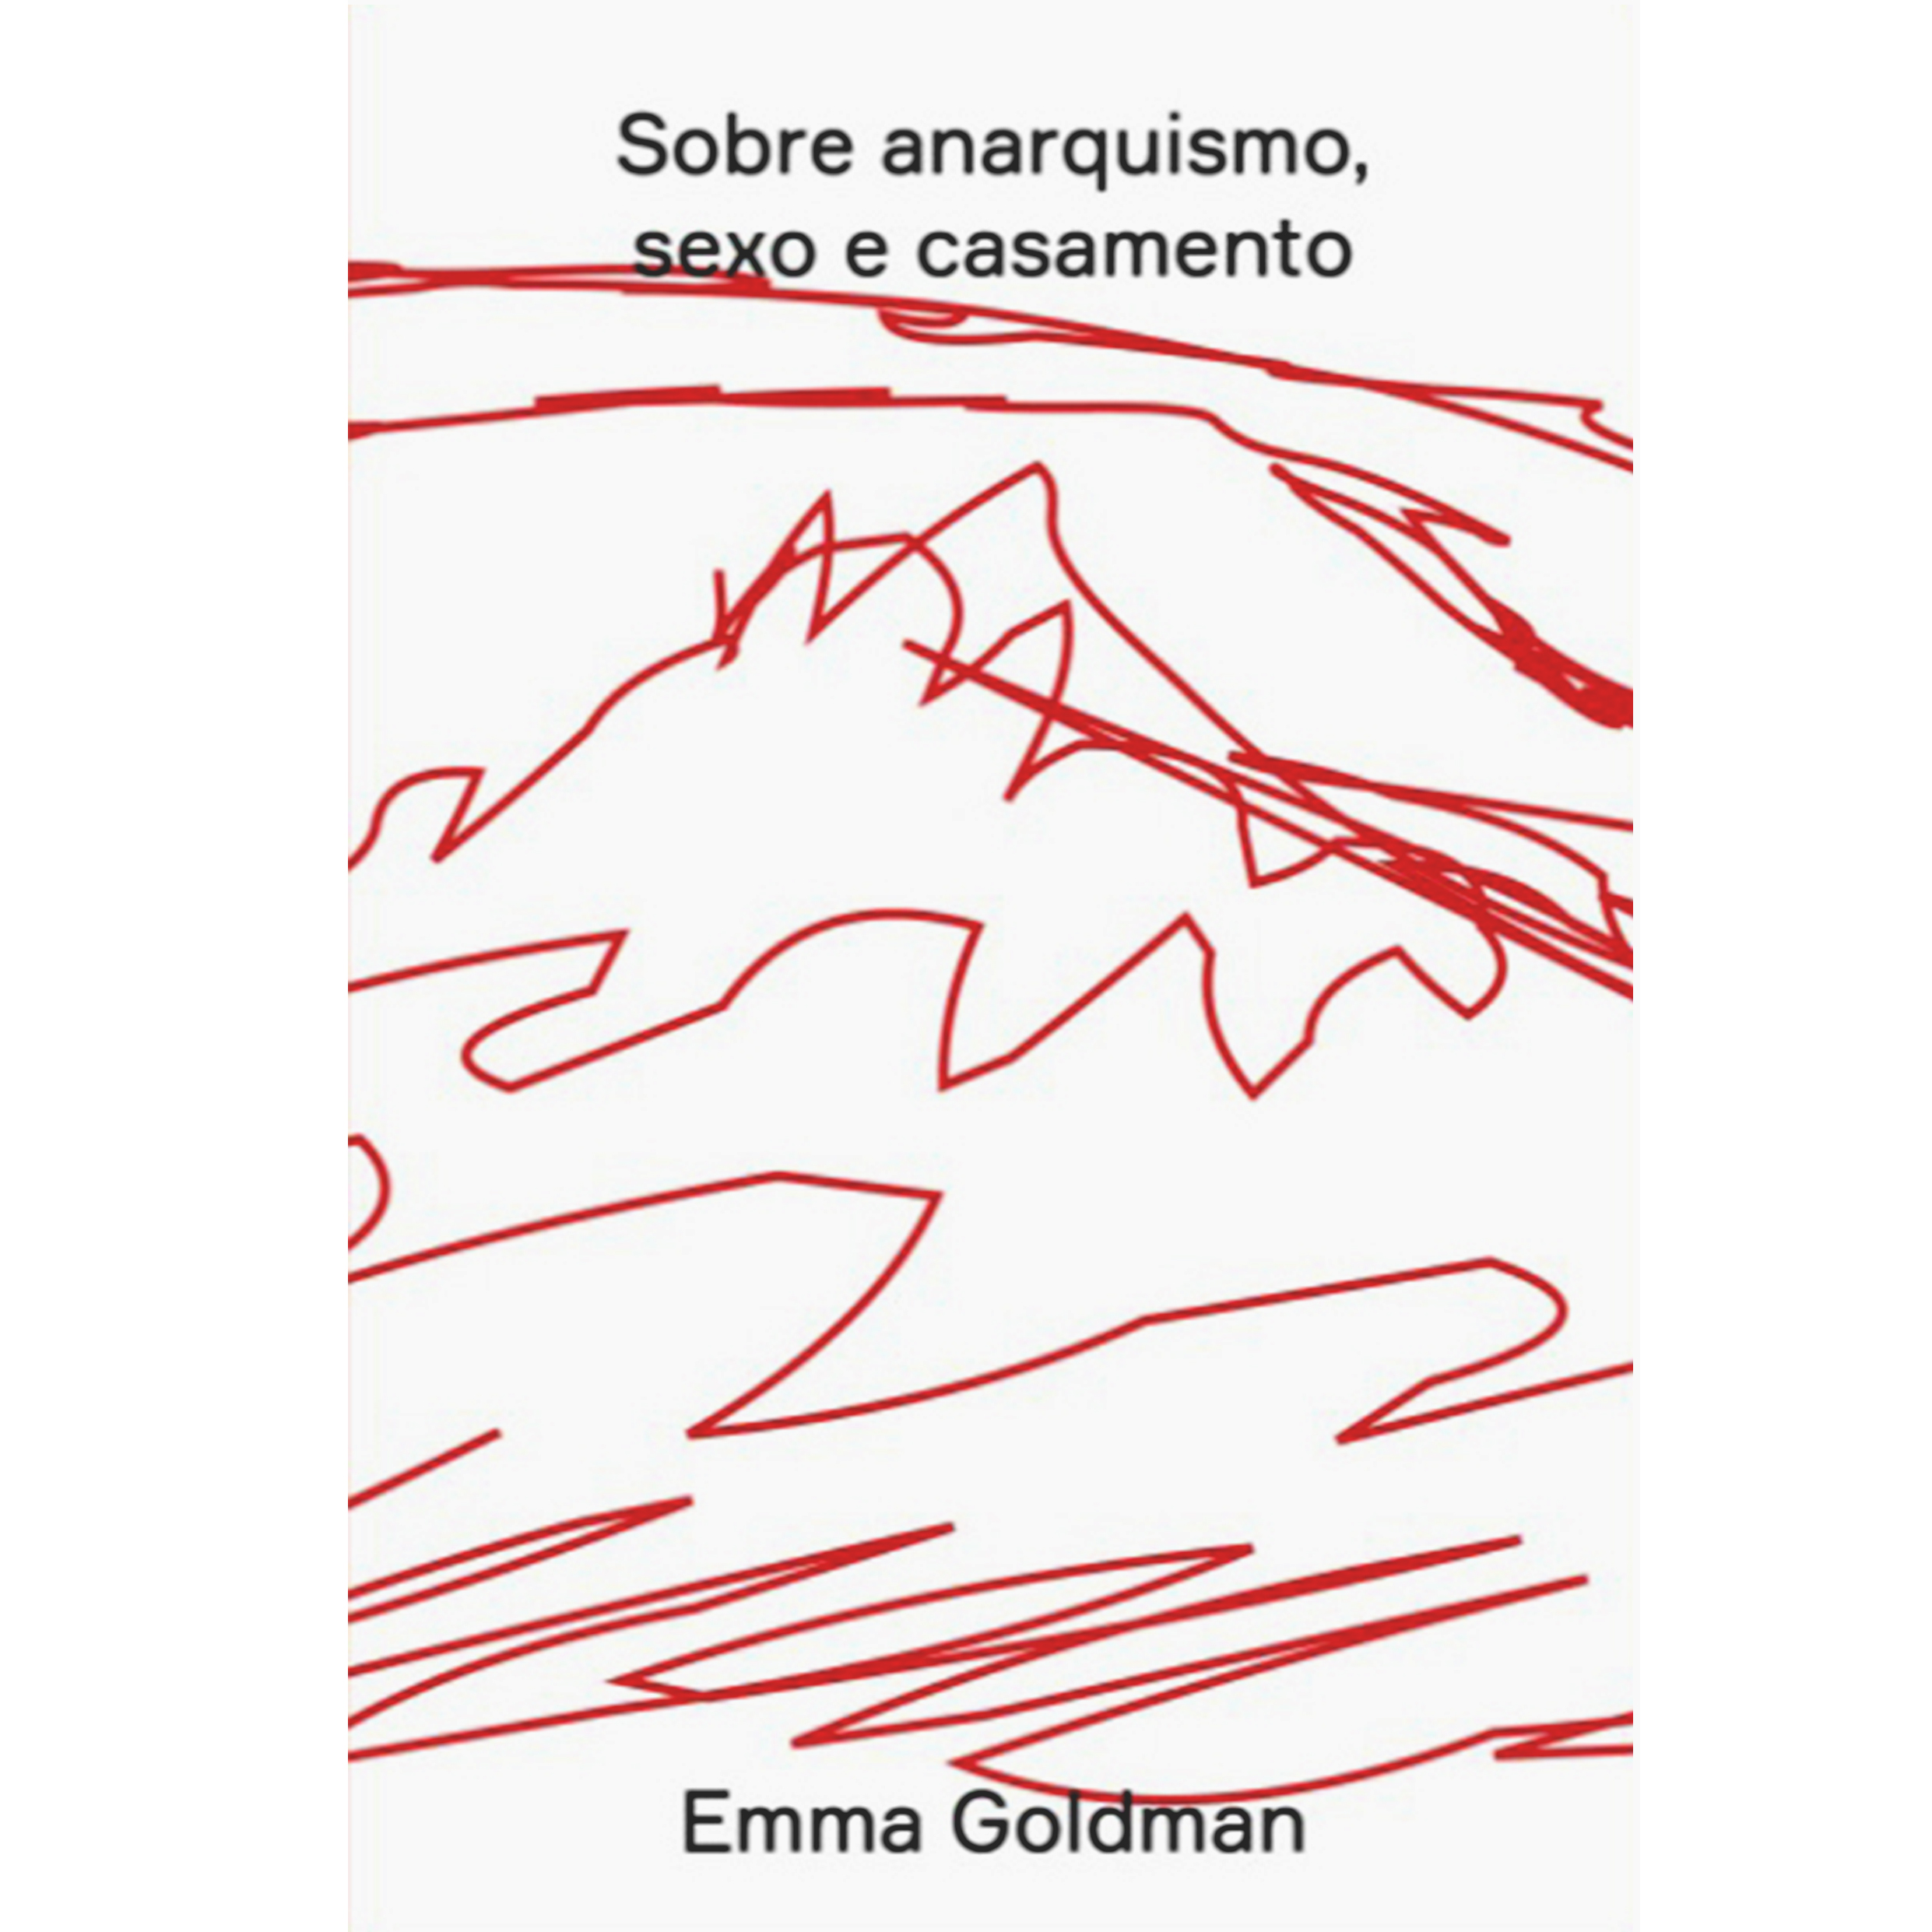
\includegraphics[width=74mm]{./grid/goldman.jpg}
\end{center}

\hspace*{-7cm}\hrulefill\hspace*{-7cm}

\medskip

\noindent{}Sob perspectiva da implacável anarquista que foi Emma Goldman, \textit{Sobre anarquismo, sexo e casamento} \hlc{trata de temas como o controle de natalidade, o puritanismo norte-americano, a repressão sexual, o amor livre, o ciúme, a prostituição, a homossexualidade, a desigualdade entre os sexos, a maternidade, a emancipação feminina, o movimento sufragista na Inglaterra e Estados Unidos e a trajetória de uma série de mulheres extraordinárias}, dentre elas heroínas e mártires do movimento revolucionário russo. 

O contexto no qual esses textos foram escritos passou pela Primeira Guerra Mundial, a Revolução Russa e a ascensão do fascismo italiano e do nacional-socialismo na Alemanha. Dada a sua condição de russa, judia, anarquista e crítica implacável do puritanismo estadunidense à autocracia soviética, tornavam-lhe ainda mais vulnerável --- dos Estados Unidos à Rússia, e nos mais diferentes círculos.


\vfill

\noindent\begin{minipage}[c]{.5\linewidth}
{\small\textbf{
\hspace*{-.1cm}Editora: Hedra\\
Título: Sobre anarquismo, sexo e casamento\\
Autor: Emma Goldman\\ 
ISBN: 978-65-89705-23-9\\
Páginas: 250 (provisório)\\
Formato: 13,3x21\,cm\\
Preço: R\$ 69,90\\
}}
\end{minipage}

\pagebreak


\begin{center}
\hspace*{-3.6cm}\raisebox{5cm}{\rotatebox[origin=t]{90}{\huge\textbf{Lançamento}}}
\hspace*{3.1cm}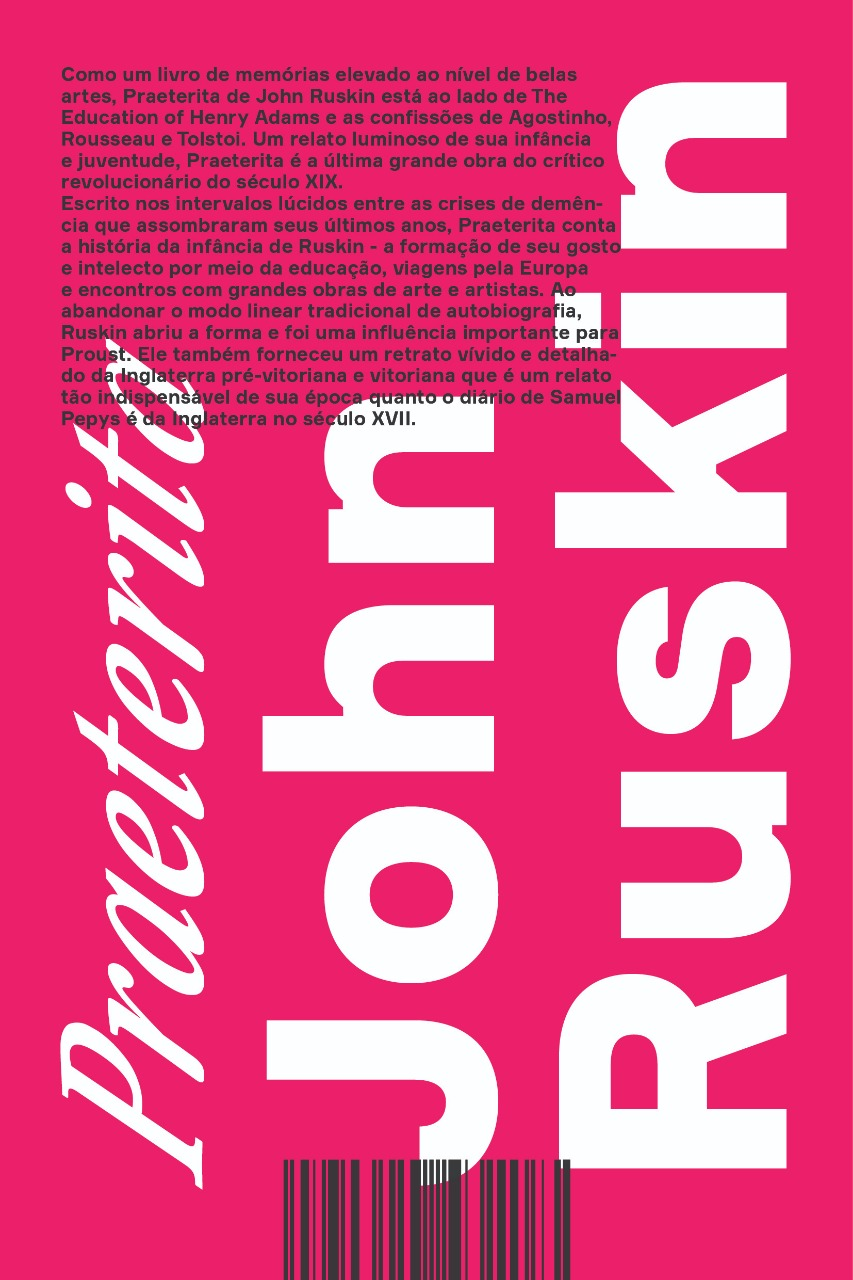
\includegraphics[width=74mm]{./grid/ruskin.jpg}
\end{center}

\hspace*{-7cm}\hrulefill\hspace*{-7cm}

\medskip

\noindent{}John Ruskin (1819--1900), \hlc{foi um dos mais importantes intelectuais da era vitoriana. Principal teórico da preservação arquitetônica e ambiental da Inglaterra do século \textsc{xix} e crítico perspicaz das transformações sociais trazidas ao país pela industrialização, a qual veementemente combateu. Excêntrico, vinculado ao romantismo, grande esteta, valorizava a sensibilidade subjetiva em contraponto à razão}; contraditório --- ao mesmo tempo aristocrático, reacionário e simpático ao socialismo. \textit{Praeterita}, sua autobiografia, foi sua última obra e testamento literário. Escrita ao longo de 27 anos, a desigualdade de suas partes reflete o estado mental do autor durante o período de sua elaboração. O livro, heterodoxo como gênero e de caráter ``experimental'', não segue os modelos de autobiografias então vigentes --- geralmente apresentados em termos de confissão religiosa ---, e poderia também ser considerado como narrativa de viagem, elegia, memória filial ou coleção de excertos de diários. Esta tradução contempla apenas o primeiro dos três volumes de \textit{Praeterita}.

\vfill

\noindent\begin{minipage}[c]{1\linewidth}
{\small\textbf{
\hspace*{-.1cm}Editora: Hedra\\
Título: Praeterita\\
Autor: John Ruskin\\ 
ISBN: 978-65-89705-24-6\\
Páginas: 250 (provisório)\\
Formato: 13,3x21\,cm\\
Preço: R\$ 69,90\\
}}
\end{minipage}

\pagebreak

\begin{center}
\hspace*{.5cm}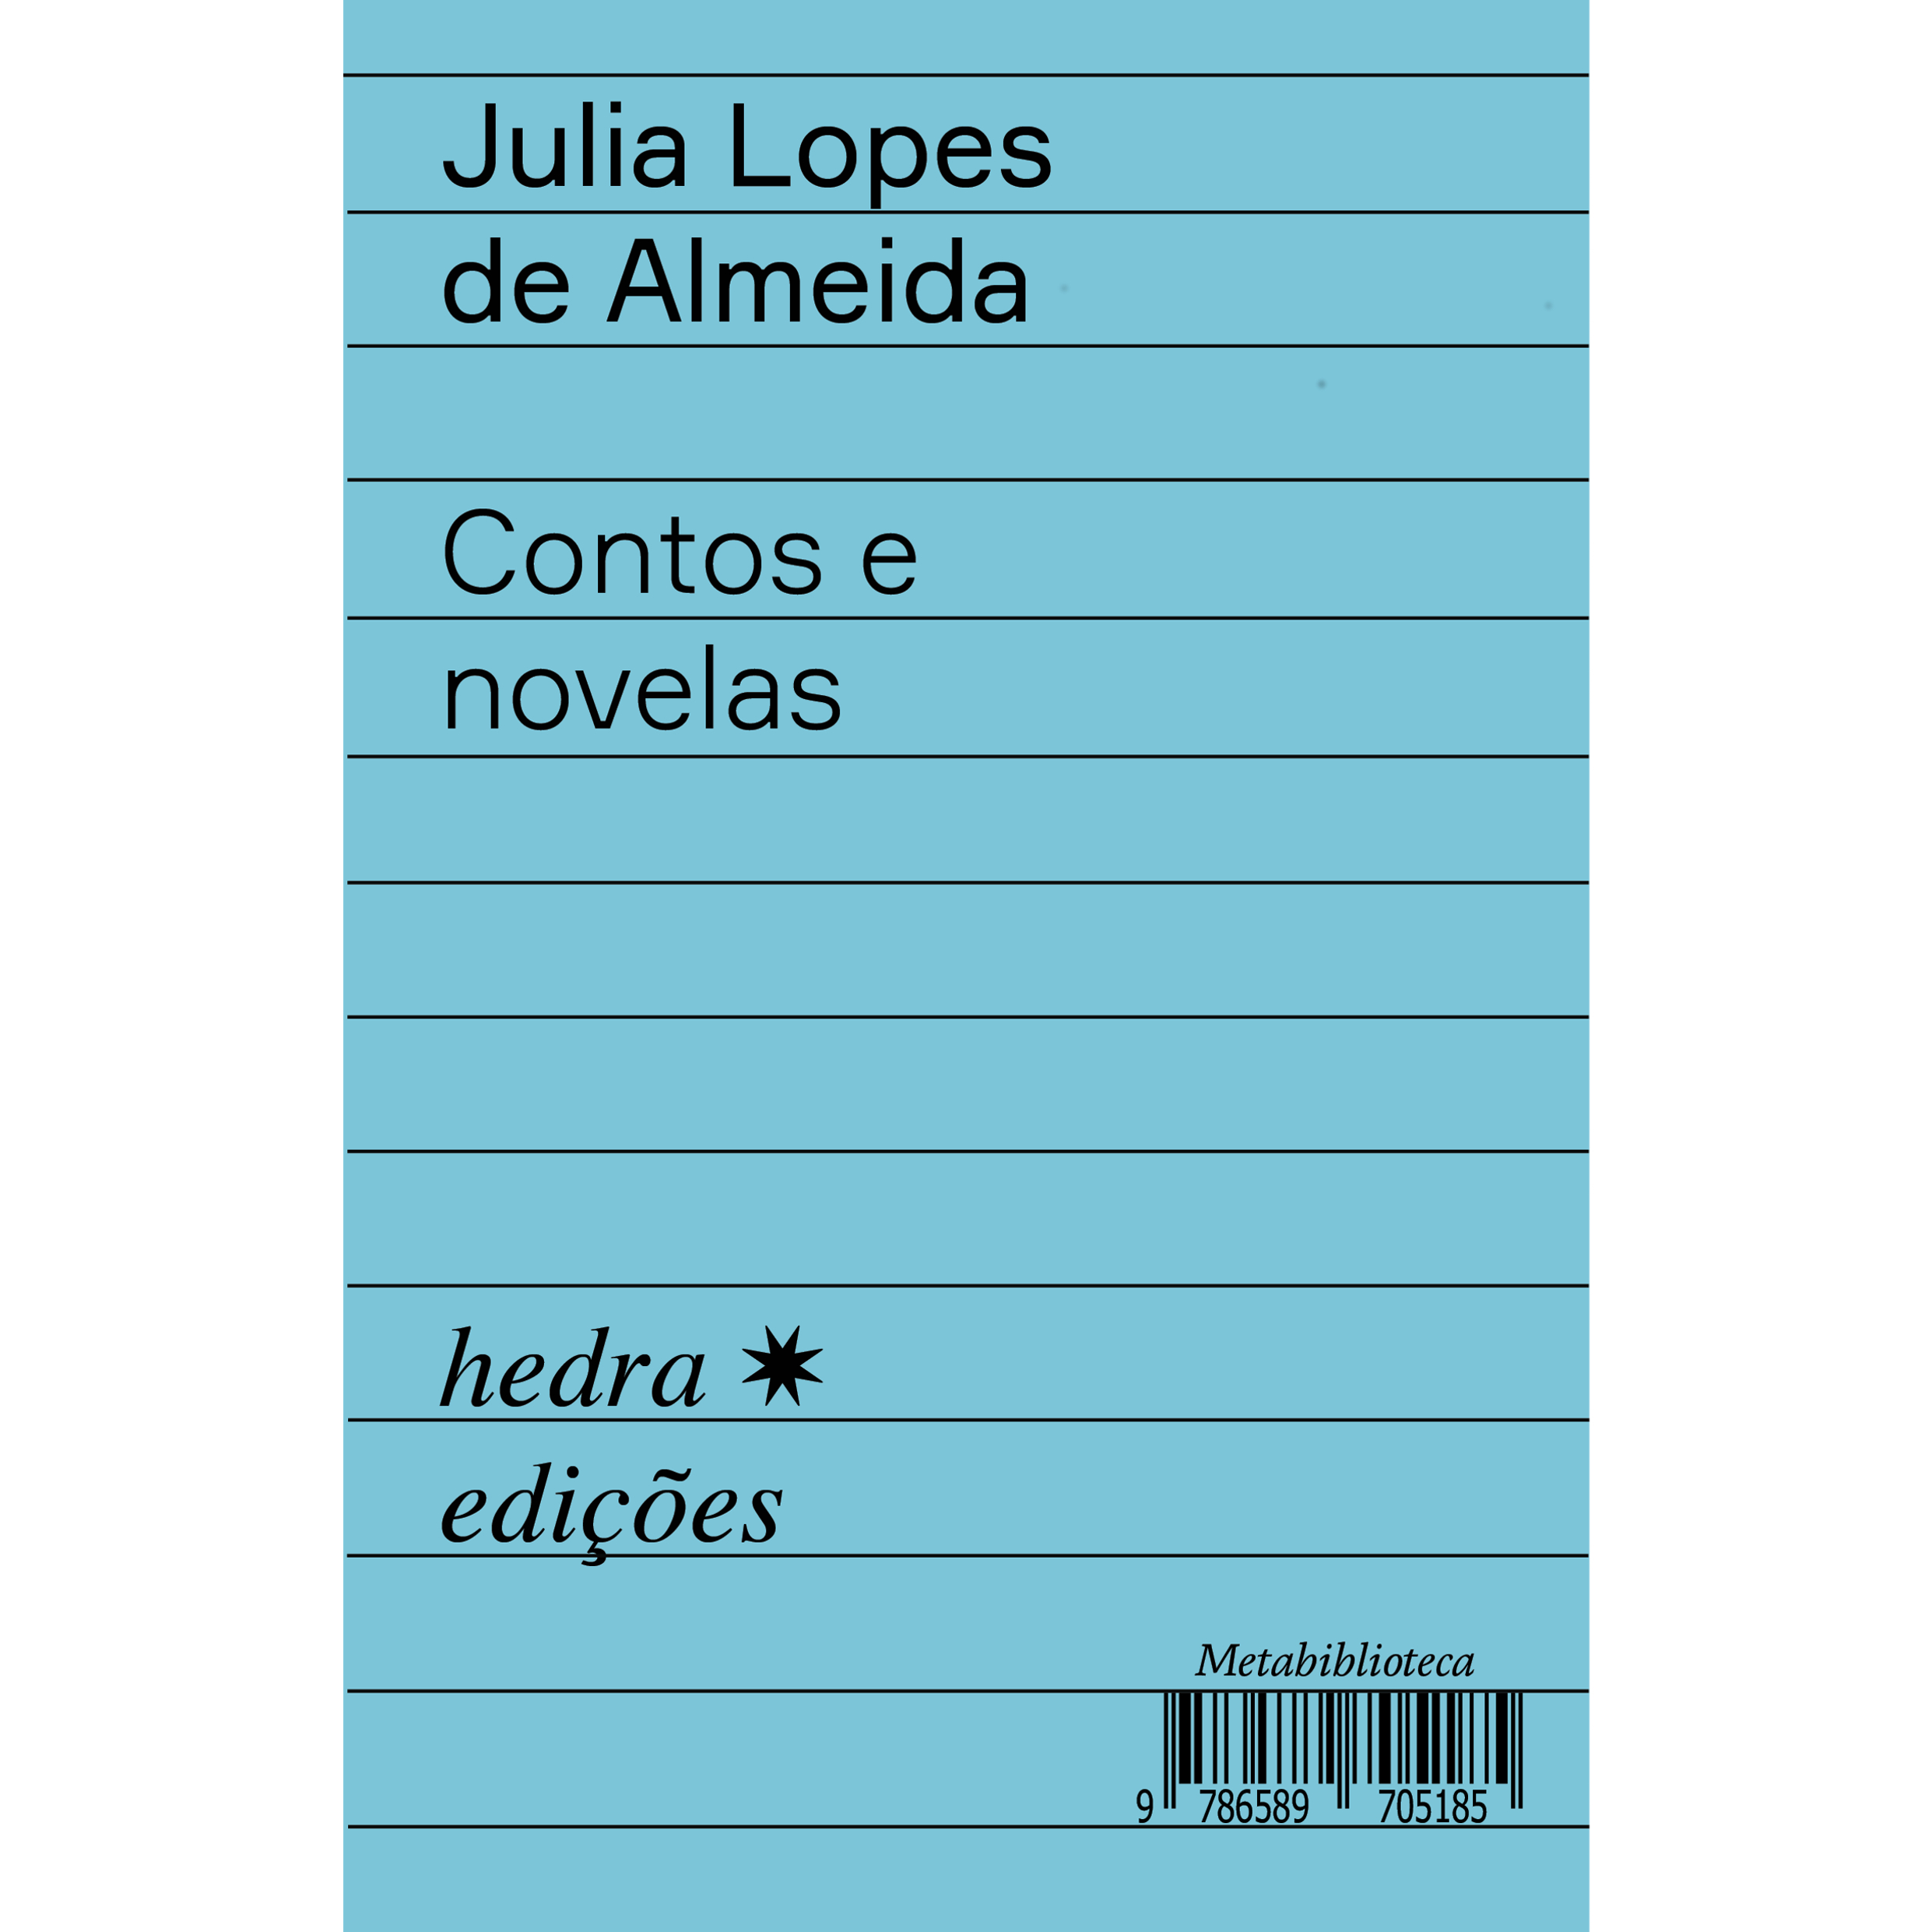
\includegraphics[width=74mm]{./grid/almeida.jpg}
\end{center}

\hspace*{-7cm}\hrulefill\hspace*{-7cm}

\medskip

\noindent{}O livro \textit{Contos e novelas} é uma antologia de narrativas curtas de Júlia Lopes de Almeida, extraídas de duas de suas obras, \textit{Ânsia eterna} (1903) e \textit{A isca} (1922), em que a escritora apresenta alguns dos \hlc{principais elementos que caracterizam sua literatura, como a presença do insólito, o lugar da mulher na sociedade patriarcal, os conflitos familiares, as marcas da escravidão e os contrastes sociais, políticos e econômicos, resultantes da modernização}. Embora não sejam os únicos volumes de narrativas curtas da escritora, esses dois livros foram selecionados por apresentarem algumas das características da narrativa de Júlia Lopes e temas que permeiam sua obra.

\vfill

\noindent\begin{minipage}[c]{1\linewidth}
{\small\textbf{
\hspace*{-.1cm}Editora: Hedra\\
Título: Contos e novelas\\
Autor: Júlia Lopes de Almeida\\ 
ISBN: 978-65-89705-26-0\\
Páginas: 190 (provisório)\\
Formato: 13,3x21\,cm\\
Preço: R\$ 57,90\\
}}
\end{minipage}

\pagebreak


\begin{center}
\hspace*{-3.6cm}\raisebox{5cm}{\rotatebox[origin=t]{90}{\huge\textbf{Lançamento}}}
\hspace*{3.1cm}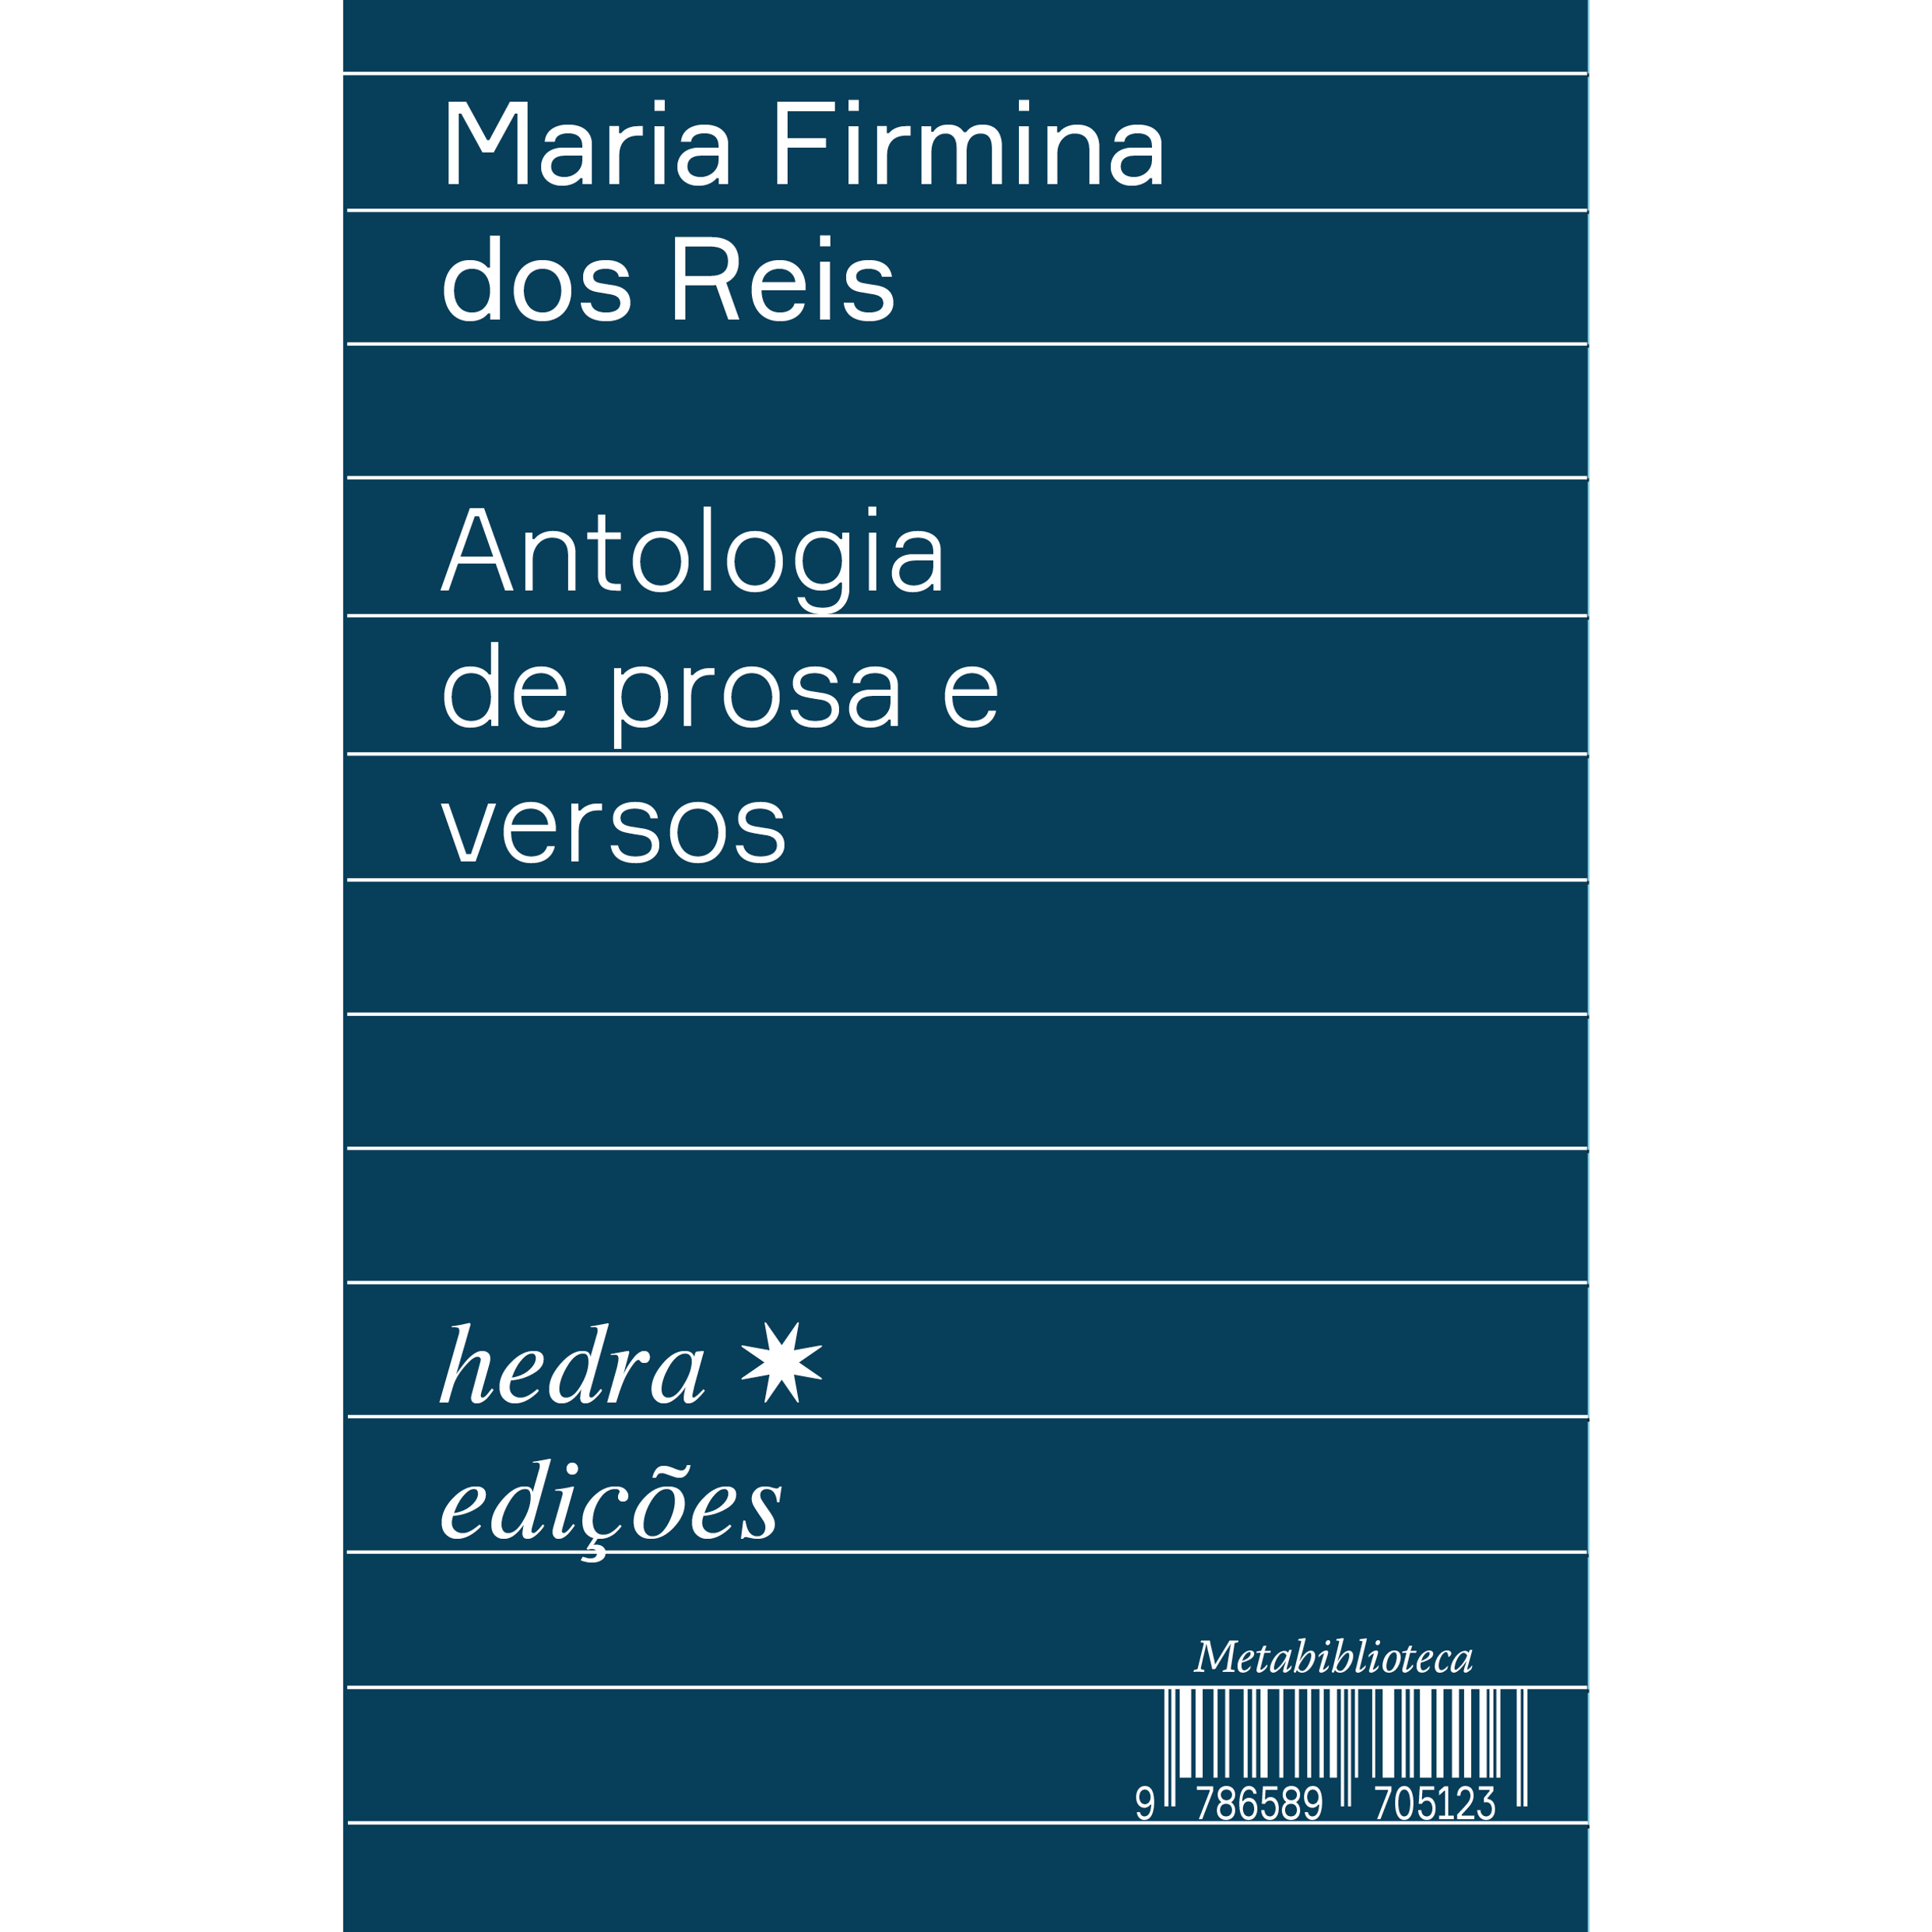
\includegraphics[width=74mm]{./grid/firmina.jpg}
\end{center}

\hspace*{-7cm}\hrulefill\hspace*{-7cm}

\medskip

\noindent{}\hlc{Maria Firmina dos Reis é considerada a primeira romancista negra da história da literatura brasileira e sua obra foi resgatada apenas na segunda metade do século \textsc{xx}}. \textit{Antologia de prosa e versos} reúne textos de diversos gêneros de Maria Firmina dos Reis, como o conto ``A escrava'', a novela ``Gupeva'' e poemas extraídos das obras \textit{Cantos à beira-mar} e \textit{Parnaso maranhense}, além de outras coletâneas mais recentes da autora. Nesta antologia, a escritora apresenta alguns dos principais elementos que caracterizam sua literatura, como a condição dos escravizados, que passam a ter protagonismo nas narrativas, o papel da mulher na sociedade, as condições dos povos indígenas, um sentimentalismo romântico amoroso e a exaltação da terra.
\vfill

\noindent\begin{minipage}[c]{1\linewidth}
{\small\textbf{
\hspace*{-.1cm}Editora: Hedra\\
Título: Antologia de prosa e versos\\
Autor: Maria Firmina dos Reis\\ 
ISBN: 978-65-89705-25-3\\
Páginas: 162 (provisório)\\
Formato: 13,3x21\,cm\\
Preço: R\$ 50,00\\
}}
\end{minipage}

\pagebreak

\begin{center}
\hspace*{.5cm}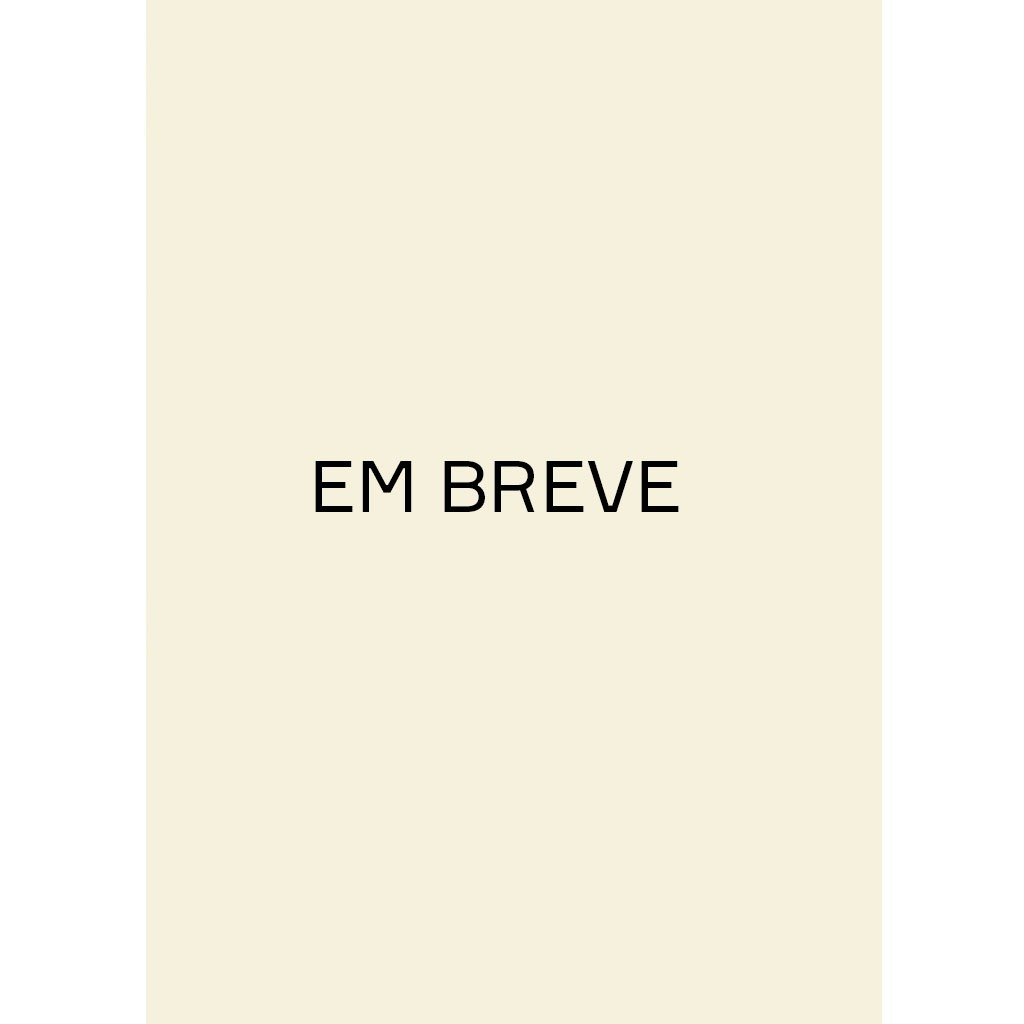
\includegraphics[width=74mm]{./grid/breve.jpeg}
\end{center}

\hspace*{-7cm}\hrulefill\hspace*{-7cm}

\medskip

\noindent{}As relações sociais passaram a figurar cada vez mais em ambientes digitais. Os rastros dessas ações se transformaram em elementos cruciais para controle e disputas econômicas, políticas e culturais do início do século \textsc{xxi}. É o chamado capitalismo informacional, baseado na coleta, monitoramento e análise de dados pessoais. Dados que, se deveriam circular livremente em redes distribuídas globalmente, têm sido coletados constantemente e utilizados sem que saibamos como e por quê e, em grande parte, fora de qualquer regulamentação. \hlc{É neste cenário que as  corporações têm se apropriado da tecnologia para se colocar à frente da concorrência, ao passo que Estados e governos as usam como dispositivos de controle sobre os cidadãos}. Para compreender esse fenômeno, pesquisadoras e pesquisadores se propõem a analisar neste livro as tensões da sociedade de controle, se apoiando nas contribuições de Gilbert Simondon, Félix Guattari, Gilles Deleuze, Maurizio Lazzarato, Michel Foucault, Manuel Castells, Frank Pasquale, Shoshana Zuboff, entre outros.

\vfill

\noindent\begin{minipage}[c]{1\linewidth}
{\small\textbf{
\hspace*{-.1cm}Editora: Hedra\\
Título: A sociedade de controle: manipulação\\ e modulação nas redes digitais\\
Autor: Joyce Souza, Rodolfo Avelino e Sérgio Amadeu da Silveira\\ 
ISBN: 978-65-89705-19-2\\
Páginas: 160 (provisório)\\
Formato: 12,7x19,1\,cm\\
Preço: R\$ 54,00\\
}}
\end{minipage}

\pagebreak

\begin{center}
\hspace*{.5cm}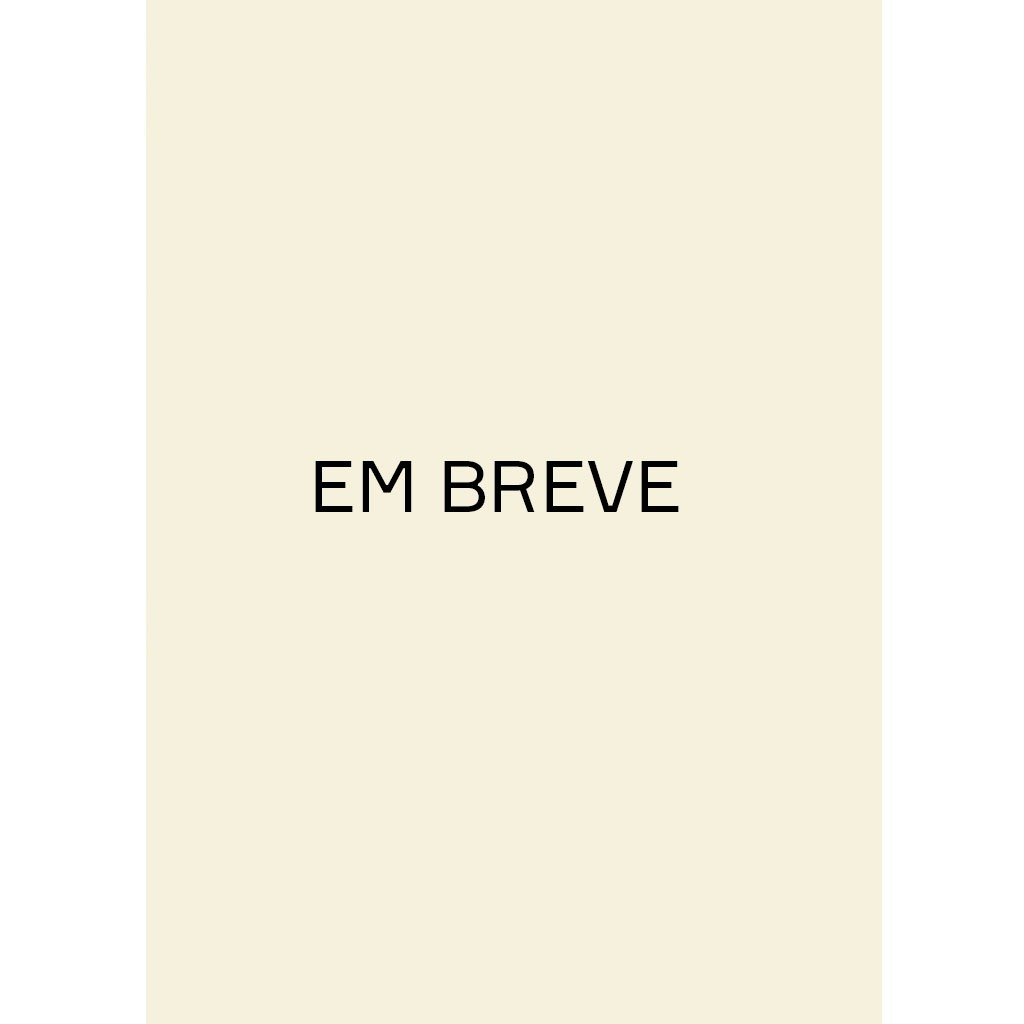
\includegraphics[width=74mm]{./grid/breve.jpeg}
\end{center}

\hspace*{-7cm}\hrulefill\hspace*{-7cm}

\medskip

\noindent{}Inserir.

\vfill

\noindent\begin{minipage}[c]{1\linewidth}
{\small\textbf{
\hspace*{-.1cm}Editora: Hedra\\
Título: Política, ativismo e cultura na era das redes digitais\\
Autor: Sérgio Amadeu da Silveira\\ 
ISBN: Inserir.\\
Páginas: Inserir.\\
Formato: 12,7x19,1\,cm\\
Preço: R\$ Inserir.\\
}}
\end{minipage}

\pagebreak

\begin{center}
\hspace*{.5cm}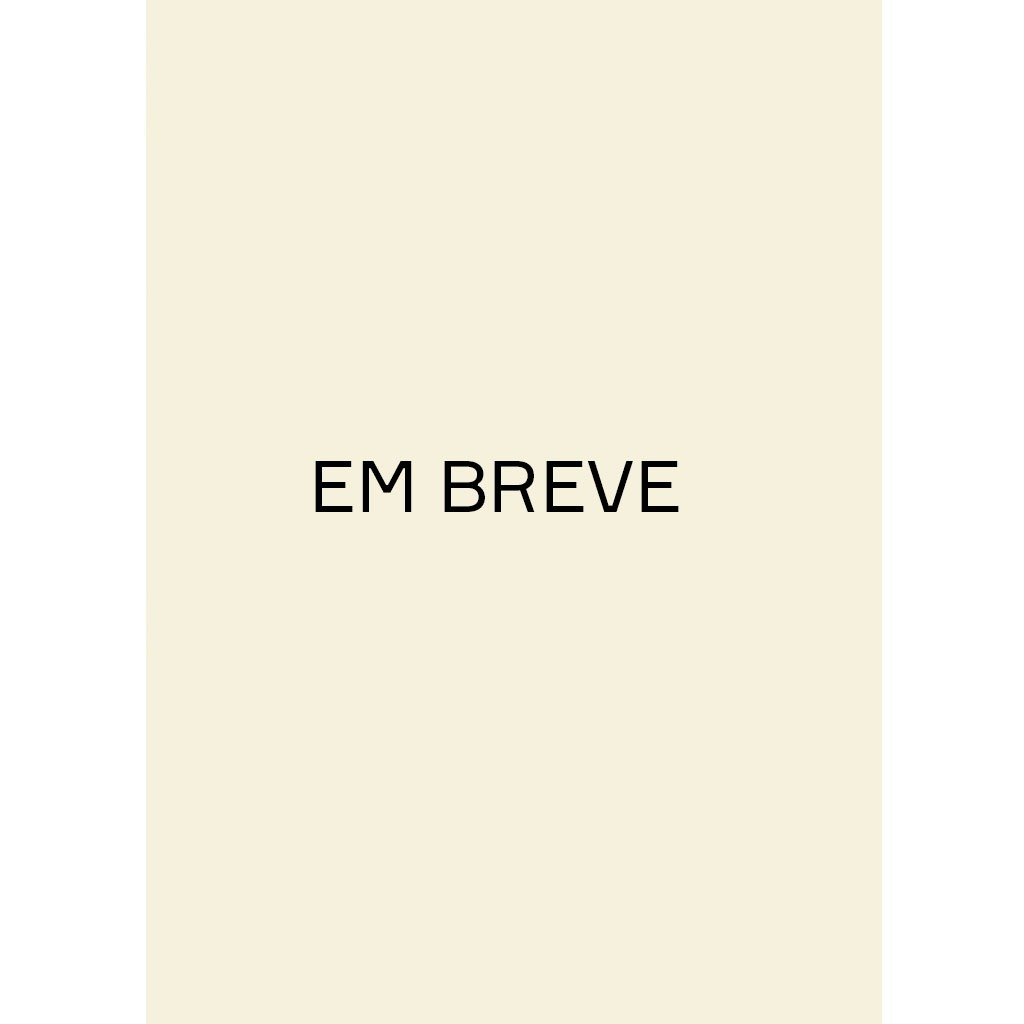
\includegraphics[width=74mm]{./grid/breve.jpeg}
\end{center}

\hspace*{-7cm}\hrulefill\hspace*{-7cm}

\medskip

\noindent{}Inserir.

\vfill

\noindent\begin{minipage}[c]{1\linewidth}
{\small\textbf{
\hspace*{-.1cm}Editora: Hedra\\
Título: Câmara escuro\\
Autor: Moacir Amâncio\\ 
ISBN: Inserir.\\
Páginas: Inserir.\\
Formato: Inserir.\\
Preço: R\$ Inserir.\\
}}
\end{minipage}

\pagebreak

\vspace*{1.5cm}

\noindent{}{\nohyphens{\LARGE{Texto}}}

\bigskip

\hfill{}\scalebox{.8}{AUTOR}

\bigskip
\bigskip
\bigskip

\begin{multicols}{2}
\noindent{}Mussum Ipsum, cacilds vidis litro abertis. Atirei o pau no gatis, per gatis num morreus. Leite de capivaris, leite de mula manquis sem cabeça. Praesent malesuada urna nisi, quis volutpat erat hendrerit non. Nam vulputate dapibus. Suco de cevadiss, é um leite divinis, qui tem lupuliz, matis, aguis e fermentis.

Tá deprimidis, eu conheço uma cachacis que pode alegrar sua vidis. Suco de cevadiss deixa as pessoas mais interessantis. In elementis mé pra quem é amistosis quis leo. Quem num gosta di mim que vai caçá sua turmis!

Viva Forevis aptent taciti sociosqu ad litora torquent. Mauris nec dolor in eros commodo tempor. Aenean aliquam molestie leo, vitae iaculis nisl. Posuere libero varius. Nullam a nisl ut ante blandit hendrerit. Aenean sit amet nisi. Vehicula non. Ut sed ex eros. Vivamus sit amet nibh non tellus tristique interdum.

Em pé sem cair, deitado sem dormir, sentado sem cochilar e fazendo pose. Detraxit consequat et quo num tendi nada. Pra lá , depois divoltis porris, paradis. Per aumento de cachacis, eu reclamis.

Quem manda na minha terra sou euzis! A ordem dos tratores não altera o pão duris. Paisis, filhis, espiritis santis. Aenean aliquam molestie leo, vitae iaculis nisl.

Diuretics paradis num copo é motivis de denguis. Mais vale um bebadis conhecidiss, que um alcoolatra anonimis. Sapien in monti palavris qui num significa nadis i pareci latim. Admodum accumsan disputationi eu sit. Vide electram sadipscing et per.

Manduma pindureta quium dia nois paga. Interagi no mé, cursus quis, vehicula ac nisi. Praesent vel viverra nisi. Mauris aliquet nunc non turpis scelerisque, eget. Casamentiss faiz malandris se pirulitá.

Quem num gosta di mé, boa gentis num é. Si num tem leite então bota uma pinga aí cumpadi! Todo mundo vê os porris que eu tomo, mas ninguém vê os tombis que eu levo! Cevadis im ampola pa arma uma pindureta.

\vspace{\baselineskip}

{\small\fakereceipt{
\noindent{}Diuretics paradis num copo é motivis de denguis. Mais vale um bebadis conhecidiss, que um alcoolatra anonimis. Sapien in monti palavris qui num significa nadis i pareci latim. Admodum accumsan disputationi eu sit. Vide electram sadipscing et per.
}}

\vspace{\baselineskip}

Mussum Ipsum, cacilds vidis litro abertis. Atirei o pau no gatis, per gatis num morreus. Leite de capivaris, leite de mula manquis sem cabeça. Praesent malesuada urna nisi, quis volutpat erat hendrerit non. Nam vulputate dapibus. Suco de cevadiss, é um leite divinis, qui tem lupuliz, matis, aguis e fermentis.

Tá deprimidis, eu conheço uma cachacis que pode alegrar sua vidis. Suco de cevadiss deixa as pessoas mais interessantis. In elementis mé pra quem é amistosis quis leo. Quem num gosta di mim que vai caçá sua turmis!

Viva Forevis aptent taciti sociosqu ad litora torquent. Mauris nec dolor in eros commodo tempor. Aenean aliquam molestie leo, vitae iaculis nisl. Posuere libero varius. Nullam a nisl ut ante blandit hendrerit. Aenean sit amet nisi. Vehicula non. Ut sed ex eros. Vivamus sit amet nibh non tellus tristique interdum.

Em pé sem cair, deitado sem dormir, sentado sem cochilar e fazendo pose. Detraxit consequat et quo num tendi nada. Pra lá , depois divoltis porris, paradis. Per aumento de cachacis, eu reclamis.

Quem manda na minha terra sou euzis! A ordem dos tratores não altera o pão duris. Paisis, filhis, espiritis santis. Aenean aliquam molestie leo, vitae iaculis nisl.

Diuretics paradis num copo é motivis de denguis. Mais vale um bebadis conhecidiss, que um alcoolatra anonimis. Sapien in monti palavris qui num significa nadis i pareci latim. Admodum accumsan disputationi eu sit. Vide electram sadipscing et per.

Manduma pindureta quium dia nois paga. Interagi no mé, cursus quis, vehicula ac nisi. Praesent vel viverra nisi. Mauris aliquet nunc non turpis scelerisque, eget. Casamentiss faiz malandris se pirulitá.

Quem num gosta di mé, boa gentis num é. Si num tem leite então bota uma pinga aí cumpadi! Todo mundo vê os porris que eu tomo, mas ninguém vê os tombis que eu levo! Cevadis im ampola pa arma uma pindureta.

\bigskip

\noindent{}\textcolor{gray}{\footnotesize\slsc{\textls[-15]{Texto tal tal e tal.}}}
\end{multicols}

\pagebreak
\pagestyle{hedracat}

\begin{multicols}{2}
\begin{enumerate}
\raggedright\nohyphens{
\item Ecopolítica, \textbf{Edson Passetti (org.)}	
\item Mare nostrum: Paranã Tipi, \textbf{Fabio Atui}
\item Crônicas de caça e criação, \textbf{Uirá Garcia}
\item Nas redes guarani, \textbf{Valéria Macedo}
\item A constituição traída, \textbf{Cleonildo Cruz (org.)}
\item Diário de um escritor na Rússia, \textbf{Flávio Ricardo Vassoler}
\item Lugar de negro, lugar de branco?, \textbf{Douglas Rodrigues Barros}
\item A sociedade de controle, \textbf{Sergio Amadeu (org.)}
\item O renascimento do autor, \textbf{Caio Gagliardi}
\item O que eu vi o que nós veremos, \textbf{Santos Dumont}
\item O outro lado da moeda (Teleny), \textbf{Oscar Wilde}
\item Imagens de um mundo trêmulo, \textbf{John Milton}
\item Michel Temer e o fascismo comum, \textbf{Tales Ab'Sáber}
\item Ao longo do rio, \textbf{Alexandre Koji Shiguehara}
\item Solombra, ou a sombra que cai sobre o eu, \textbf{João Adolfo Hansen}
\item Joana d'Arc, \textbf{Jules Michelet}
\item O coletivo aleatório, \textbf{Luis Marra}
\item A história das religiões na cultura moderna, \textbf{Marcello Massenzio}
\item Cordel - F. das Chagas Batista, \textbf{Francisco das Chagas Batista}
\item Elixir do pajé, \textbf{Bernardo Guimarães}
\item Cordel - João Martins de Athayde, \textbf{João Martins de Athayde}
\item Modos de representação da Bienal de São Paulo, \textbf{Vinicius Spricigo}
\item Padeirinho da Mangueira: retrato sincopado de um artista, \textbf{Franco Paulino}
\item Do futuro e da morte do teatro brasileiro, \textbf{Christina Barros Riego}
\item Canudos, história em versos, \textbf{Manuel Pedro das Dores Bombinho}
\item O cego e outros contos, \textbf{D. H. Lawrence}
\item Poesia seiscentista
\item Monoteísmos e dualismos: as religiões da salvação, \textbf{Giovanni Filoramo}
\item Apologia de Galileu, \textbf{Tommaso Campanella}
\item Flor do deserto, \textbf{Waris Dirie; Cathleen Miller}
\item Cinco lugares da fúria, \textbf{Pádua Fernandes}
\item O livro dos mandamentos, \textbf{Maimônides}
\item A conjuração de Catilina, \textbf{Salústio}
\item Fábula de Polifemo e Galatéia e outros poemas, \textbf{Góngora}
\item Histórias de igrejas destruídas, \textbf{Eduardo Brigagão Verderame}
\item Performances, \textbf{Brian Friel}
\item Cultura pop japonesa, \textbf{Sonia Bide Luyten}
\item História trágica do doutor Fausto, \textbf{Christopher Marlowe}
\item Micromegas, \textbf{Voltaire}
\item Politeísmos: as religiões do mundo antigo, \textbf{Paolo Scarpi}
\item Triunfos, \textbf{Petrarca}
\item Museu arte hoje, \textbf{Martin Grossmann; Gilberto Mariotti}
\item Viagem sentimental, \textbf{Laurence Sterne}
\item A Arte de olhar diferente, \textbf{Braulio Tavares}
\item O Pequeno Zacarias chamado Cinábrio, \textbf{E.T.A. Hoffman}
\item Oliver Twist (Bolso), \textbf{Charles Dickens}
\item Alegoria - Construção e interpretação da metáfora, \textbf{João Adolfo Hansen}
\item Teatro do êxtase, \textbf{Fernando Pessoa}
\item Paulo Whitaker, \textbf{Paulo Whitaker}
\item Todas as coisas pequenas, \textbf{Noemi Jaffe}
\item Questão do fim da arte em Hegel, \textbf{Marco Aurélio Werle}
\item Tratados da terra e gente do Brasil, \textbf{Fernão Cardim}
\item Dos nervos, \textbf{Ricardo Lísias}
\item Adeus ponta do meu nariz, \textbf{Edward Lear}
\item Cidade ampliada, \textbf{Rodrigo José Fermino}
\item O diário perdido do Jardim Maia, \textbf{Luís Marra}
\item Sobre a filosofia e outros diálogos, \textbf{Jorge Luis Borges; Osvaldo Ferrari}
\item Cordel: Franklin Maxado, \textbf{Franklin Maxado}
\item Dos novos sistemas na arte, \textbf{Kazimir Malievitch}
\item Cordel: Cuíca de Santo Amaro, \textbf{Cuíca de Santo Amaro}
\item Manual da destruição, \textbf{Alexandre Dal Farra}
\item A imprensa carnavalesca no Brasil, \textbf{José Ramos Tinhorão}
\item Índia e Extremo Oriente: via da libertação e da imortalidade, \textbf{Massimo Raveri}
\item Leitores e leituras de Clarice Lispector
\item Círculos de coca e fumaça, \textbf{Danilo Paiva Ramos}
\item Cordel: Severino José, \textbf{Severino José}
\item Escritório; O Espaço da Produção, \textbf{Claudio Silveira Amaral}
\item As minas de Salomão, \textbf{Rider Haggard}
\item Crédito à morte, \textbf{Anselm Jappe}
\item A cidade e as serras, \textbf{Eça de Queiroz}
\item Oliver Twist, \textbf{Charles Dickens}
\item Dao De Jing, \textbf{Lao Zi}
\item Sobre a amizade e outros diálogos, \textbf{Jorge Luis Borges; Osvaldo Ferrari}
\item Aqui tem coisa, \textbf{Patativa do Assaré}
\item Dicionário livre do santome-português, \textbf{Araújo \& Hagemeijer}
\item Aqui tem coisa, \textbf{Patativa do Assaré}
\item Imagem contemporânea I
\item Cordel - J. Borges, \textbf{José Francisco Borges}
\item Exato acidente, \textbf{Tony Monti}
\item Woyzeck, \textbf{George Buchner}
\item Autobiografia de um super-herói, \textbf{Alexandre Barbosa de Souza}
\item O menino da rosa, \textbf{Tony Monti}
\item Cordel - Rouxinol do Rinaré, \textbf{Rouxinol do Rinaré}
\item Imagem contemporânea II
\item História da província Santa Cruz, \textbf{Pero de Magalhães Gandavo}
\item Édipo Rei, \textbf{Sófocles}
\item Cordel - José Soares, \textbf{José Soares}
\item Greve contra a guerra, \textbf{Ricardo Lísias}
\item Cidade anônima, \textbf{Beatriz Furtado}
\item Primeiro de abril, \textbf{André Luiz Pinto}
\item Cordel: Oliveira de Panelas, \textbf{Oliveira de Panelas}
\item Fazendo Rizoma
\item Uma história do futebol, \textbf{Bill Murray}
\item Gangorra, \textbf{Regina Sawaya}
\item Poesia vaginal, \textbf{Glauco Mattoso}
\item Cultura popular - uma introdução, \textbf{Dominic Strinati}
\item Vocabulário de música pop, \textbf{Roy Shuker}
\item A invenção da pornografia, \textbf{Lynn Hunt}
\item Eu conheci Benny Moré
\item Deriva, \textbf{André Fernandes}
\item Fedro, \textbf{Platão}
\item Sobre os sonhos e outros diálogos, \textbf{Jorge Luis Borges; Osvaldo Ferrari}
\item O sapo voador, \textbf{Ademir Barbosa Jr.}
\item Arcana coelestia e Apocalipsis revelata, \textbf{Emanuel Swedenborg}
\item Letra de forma, \textbf{Laura Estelita Teixeira}
\item Os cães de que desistimos, \textbf{Chantal Castel}
\item Cordel - Téo Azevedo, \textbf{Téo Azevedo}
\item O que eu vi, o que nós veremos [bolso], \textbf{Santos Dumont}
\item A Fábrica de robôs, \textbf{Karel Tchápek}
\item Folhas de relva, \textbf{Walt Whitman}
\item Helio Piñon : Ideias e formas, \textbf{Pfeiffe, Helen; Ana Rosa}
\item O Rabi de Bacherach e três artigos sobre o ódio racial, \textbf{Heinrich Heine}
\item Refugiados de Idomeni, \textbf{Gabriel Bonis}
\item Visão de psicanálise, \textbf{Renato Bulcão}
\item Viagem em volta do meu quarto, \textbf{Xavier de Maistre}
\item Contos clássicos de vampiro, \textbf{Lord Byron; Bram Stoker}
\item Cultura estética e liberdade, \textbf{Friedrich Von Schiller}
\item Dostoiévski e a dialética, \textbf{Flávio Ricardo Vassoler}
\item Cabeças e outros poemas, \textbf{Pedro Luis Marques de Armas}
\item Razão sangrenta, \textbf{Robert Kurz}
\item A Velha Izerguil e outros contos, \textbf{Maksim Górki}
\item Viagem à turquia, bálcãs e Egito, \textbf{John Milton}
\item Do sentimento trágico da vida, \textbf{Miguel de Unamuno}
\item Rashômon e outros contos, \textbf{Akutagawa}
\item Feitiço de amor e outros contos, \textbf{Johann Ludwig Tieck}
\item Ode ao Vento Oeste e outros poemas, \textbf{P. B. Shelley}
\item Esperança do mundo, \textbf{Albert Camus}
\item Universidade, cidade, cidadania, \textbf{Franklin Leopoldo e Silva}
\item Estado crítico, \textbf{Régis Bonvicino}
\item Poemas da cabana montanhesa, \textbf{Saigyo}
\item Dançando em Lúnassa, \textbf{Brian Frield}
\item Lulismo, carisma pop e cultura anticrítica, \textbf{Tales Ab'Sáber}
\item Utopia Brasil, \textbf{Darcy Ribeiro}
\item Americanismo e fordismo, \textbf{Antonio Gramsci}
\item Troca de pele, \textbf{Tereza Yamashita}
\item O Surgimento da noite, \textbf{Pajés Parahiteri}
\item Contos de Sebastopol, \textbf{Liev Tolstói}
\item Um anarquista e outros contos, \textbf{Joseph Conrad}
\item Um Retrato do artista quando jovem, \textbf{James Joyce}
\item O Princípio do Estado e outros ensaios, \textbf{Mikhail Bakunin}
\item A Desmedida na medida, \textbf{Albert Camus}
\item O Chamado selvagem, \textbf{Jack London}
\item O Novo epicuro, \textbf{Edward Sellon}
\item Elogio da loucura, \textbf{Erasmo de Rotterdam}
\item Senhorita Júlia e outras peças, \textbf{August Strindberg}
\item Dublinenses, \textbf{James Joyce}
\item Don Juan ou O convidado de pedra, \textbf{Molière}
\item Manual inútil da televisão, \textbf{Paulo Henrique Amorim}
\item A Vida de Mat, \textbf{Mino Carta}
\item Baleiazzzul, \textbf{Sergio Zlotnic}
\item A Decadência do analfabetismo / A arte de birlibirloque, \textbf{José Bergamín}
\item Balada dos enforcados e outros poemas, \textbf{François Villon}
\item O Médico e o monstro, \textbf{Robert Louis Stevenson}
\item Marco Cornélio Frontão, \textbf{Pascal Quignard}
\item O Casamento do Céu e do Inferno, \textbf{William Blake}
\item O Homem da cabeça de papelão, \textbf{João do Rio}
\item Teleny, ou o reverso da medalha, \textbf{Oscar Wilde}
\item Cordel: Rodolfo Coelho Cavalcante, \textbf{Coelho Cavalcante}
\item Dicionário de História e Cultura da era Viking, \textbf{Johnni Langer}
\item Gente de Hemsö, \textbf{August Strindberg}
\item Viagem aos Estados Unidos, \textbf{Alexis de Tocqueville}
\item Sobre a utilidade e a desvantagem da história para a vida, \textbf{Friedrich Nietzsche}
\item Flossie, a Vênus de quinze anos, \textbf{Charles Swinburne}
\item Os cantos do homem-sombra
\item Escritos revolucionários, \textbf{Errico Malatesta}
\item Micromegas e outros contos, \textbf{Voltaire}
\item Descobrindo o Islã no Brasil, \textbf{Karla Lima}
\item A Cidade mágica, \textbf{Edith Nesbitt}
\item O Alienista, \textbf{Machado de Assis}
\item Cadeira de balanço, \textbf{Vanessa Campos Rocha; Flávio Castellan}
\item Inspiração nordestina, \textbf{Patativa do Assaré}
\item Coisas que a gente gosta e não gosta, \textbf{Laura Teixeira; Fábio Zimbres}
\item A Guerra começou, onde está a guerra?, \textbf{Albert Camus}
\item Poesia completa, \textbf{Orides Fontela}
\item A Volta do parafuso, \textbf{Henry James}
\item Cartas a favor da escravidão, \textbf{José de Alencar}
\item Pequeno-burgueses, \textbf{Maksim Górki}
\item Cordel : Paulo Nunes Batista, \textbf{Paulo Nunes Batista}
\item Esquimó, \textbf{Olivier Douzou}
\item Sai da frente, vaca brava!, \textbf{Ricardo Lísias}
\item Lampião... Era o cavalo do tempo atrás da besta da vida, \textbf{Antônio Klévisson Viana}
\item Cordel: Patativa do Assaré, \textbf{Patativa do Assaré}
\item Ernestine ou o nascimento do amor, \textbf{Stendhal}
\item Filadélfia, lá vou eu!, \textbf{Brian Friel}
\item Sonetos, \textbf{William Shakespeare}
\item Crônicas do crack, \textbf{Luis Marra}
\item Peixinhos, \textbf{Bruno Heitz}
\item A Última folha e outros contos, \textbf{O. Henry}
\item Contos indianos, \textbf{Stéphane Mallarmé}
\item Violência, mas para quê?, \textbf{Anselm Jappe}
\item A Vênus das peles, \textbf{Sacher-Leopold Von Masoch}
\item A Voz dos botequins e outros poemas, \textbf{Paul Verlaine}
\item Poemas, \textbf{Lord Byron}
\item A Pele do lobo e outras peças, \textbf{Artur Azevedo}
\item Explosão - Romance da etnologia, \textbf{Hubert Fichte}
\item Stephen herói, \textbf{James Joyce}
\item Diálogo imaginário entre Marx e Bakunin, \textbf{Maurice Cranston}
\item Nada ainda?, \textbf{Christian Voltz}
\item A Vênus de quinze anos (Flossie), \textbf{Charles Swinburne}
\item Os dentinhos, \textbf{Olivier Douzou}
\item Anarquismo, \textbf{Murray Bookchin}
\item Escritos sobre arte, \textbf{Charles Baudelaire}
\item Deus e o Estado, \textbf{Mikhail Bakunin}
\item Pintura e escrita do mundo flutuante, \textbf{Madalena Hashimoto Cordaro}
\item A Árvore dos cantos, \textbf{Pajés Parahiteri}
\item Poesia catalã - das origens à Guerra Civil
\item Sobre a filosofia e seu método, \textbf{Arthur Schopenhauer}
\item Pensamento político de Maquiavel, \textbf{Johann Fichte}
\item Sobre a ética, \textbf{Arthur Schopenhauer}
\item A Autobiografia do poeta-escravo, \textbf{Juan Francisco Manzano}
\item Cálcio, \textbf{Pádua Fernandes}
\item Bola de sebo e outros contos, \textbf{Guy de Maupassant}
\item Como gente grande, \textbf{Anouk Ricard}
\item O Cavalo de Ébano, \textbf{Richard Burton}
\item Nos cumes do desespero, \textbf{Emil Cioran}
\item A Vênus das peles [Bolso], \textbf{Leopold Von Sacher-Masoch}
\item Homo Pictor, \textbf{Christoph Wulf}
\item 1964
\item Desenganos da vida humana e outros poemas, \textbf{Gregório de Matos}
\item A Nostálgica e outros contos, \textbf{Aléxandros Papadiamántis}
\item Cântico dos Cânticos, \textbf{Salomão}
\item Os Sovietes traídos pelos bolcheviques, \textbf{Rudolf Rocker}
\item Autobiografia de uma pulga, \textbf{Stanislas de Rhodes}
\item Auto da barca do Inferno, \textbf{Gil Vicente}
\item A Monadologia e outros textos, \textbf{Gottfried Leibniz}
\item O Surgimento dos pássaros, \textbf{Pajés Parahiteri}
\item Contos de piratas, \textbf{Arthur Conan Doyle}
\item O Mundo ou tratado da luz, \textbf{René Descartes}
\item Manifesto comunista, \textbf{Karl Marx; Friedrich Engels}
\item Lira grega, \textbf{Giuliana Ragusa}
\item Poesia basca - das origens à Guerra Civil
\item Cordel: Klévisson Viana, \textbf{Klévisson Viana}
\item Discursos ímpios, \textbf{Marquês de Sade}
\item Cordel : Raimundo Santa Helena, \textbf{Raimundo Santa Helena}
\item Primeiro livro dos amores, \textbf{Ovídio}
\item Último reino, \textbf{Pascal Quignard}
\item Da arte de construir, \textbf{Leon Battista Alberti}
\item Frankenstein, \textbf{Mary Shelley}
\item Cordel : Zé Saldanha, \textbf{Zé Saldanha}
\item Dilma Rousseff e o ódio político, \textbf{Tales Ab'Sáber}
\item Saga dos Volsungos, \textbf{Anônimo}
\item Linear G, \textbf{Gilberto Mendonça Teles}
\item Educação e sociologia, \textbf{Émile Durkheim}
\item Histórias com dragões, príncipes e serpentes, \textbf{Vários}
\item História do boi misterioso, \textbf{Leandro Gomes de Barros; Irani Med}
\item Sobre verdade e mentira, \textbf{Friedrich Nietzsche}
\item Sermões 2, \textbf{Antônio Vieira}
\item Lisístrata, \textbf{Aristófanes}
\item Os Americanos, \textbf{Nathaniel Hawthorne; Edgar Allan Poe; Herman Melville}
\item O Sol não espera, \textbf{Marília Castello Branco}
\item O Fim do ciúme e outros contos, \textbf{Marcel Proust}
\item Álcoois, \textbf{Guillaume Apollinaire}
\item A História do planeta azul, \textbf{Andri Snaer Magnason}
\item Entre camponeses, \textbf{Errico Malatesta}
\item Ispinho e Fulô, \textbf{Patativa do Assaré}
\item Mais dia menos dia, a paixão, \textbf{Nelson de Oliveira}
\item Teogonia, \textbf{Hesíodo}
\item Ação e percepção nos processos educacionais do corpo em formação, \textbf{Cecília Noriko Ito Saito}
\item Amores e outras imagens, \textbf{Filóstrato}
\item O Fantástico reparador de feridas, \textbf{Brian Friel}
\item Mangá, \textbf{Sonia Bide Luyten}
\item Inferno, \textbf{August Strindberg}
\item Romanceiro cigano, \textbf{Sermões}
\item Sagas, \textbf{August Strindberg}
\item O Destino do erudito, \textbf{Johann Fichte}
\item Diários de Adão e Eva, \textbf{Mark Twain}
\item Habitar, \textbf{André Fernandes}
\item O Desertor, \textbf{Silva Alvarenga}
\item Os Vínculos, \textbf{Giordano Bruno}
\item O Estranho caso do Dr. Jekyll e Mr. Hyde, \textbf{Robert Louis Stevenson}
\item Sátiras, fábulas, aforismos e profecias, \textbf{Leonardo da Vinci}
\item Poesia espanhola - das origens à Guerra Civil
\item Hino a Afrodite e outros poemas, \textbf{Safo de Lesbos}
\item Revolução e liberdade, \textbf{Mikhail Bakunin}
\item Cartas do Brasil, \textbf{Antonio Vieira}
\item A Mulher que virou Tatu
\item Sermões 1, \textbf{Antônio Vieira}
\item Fé e saber, \textbf{G.W. Friedrich Hegel}
\item Negras tormentas, \textbf{Alexandre Samis}
\item Cordel: Manoel Caboclo, \textbf{Manoel Caboclo}
\item Graciliano Ramos e A Novidade, \textbf{Ieda Lebensztayn}
\item Emília Galotti, \textbf{Gotthold Ephraim Lessing}
\item Dao De Jing, \textbf{Lao Zi}
\item Histórias escondidas, \textbf{Odilon Moraes}
\item Noites egípcias e outros contos, \textbf{Aleksandr Púchikin}
\item Carmilla, a vampira de Karnstein, \textbf{Sheridan Le Fanu}
\item O desafio de Lula, \textbf{Mino Carta; Gianni Carta}
\item A Filosofia na era trágica dos gregos, \textbf{Friedrich Nietzsche}
\item O Que é bom, o que é ruim, \textbf{Vladimir Maiakóvski}
\item Em busca do Japão contemporâneo, \textbf{John Milton}
\item A Vida de H.P. Lovecraft, \textbf{S.T. Joshi}
\item A Demanda do Santo Graal, \textbf{Anônimo}
\item Trabalhos e os dias, \textbf{Hesíodo}
\item Mensagem, \textbf{Fernando Pessoa}
\item Ode sobre a melancolia e outros poemas, \textbf{John Keats}
\item O Corno de si próprio e outros contos, \textbf{Marquês de Sade}
\item Hawthorne e seus musgos, \textbf{Herman Melville}
\item Memórias de um menino judeu do Bom Retiro, \textbf{Victor Nussenzwieg}
\item No coração das trevas, \textbf{Joseph Conrad}
\item Émile e Sophie ou os solitários, \textbf{Jean-Jaqcques Rousseau}
\item Investigação sobre o entendimento humano, \textbf{David Hume}
\item Ideias de canário, \textbf{Machado de Assis}
\item Eu acuso! / O processo do capitão Dreyfus, \textbf{Émile Zola; Rui Barbosa}
\item O Livro dos dragões, \textbf{Ovídio}
\item As Bacantes, \textbf{Eurípides}
\item Contos clássicos de vampiro [Bolso], \textbf{Lord Byron; Bram Stoker}
\item Sobre a liberdade, \textbf{Stuart Mill}
\item Metamorfoses, \textbf{Ovídio}
\item O Primeiro Hamlet, \textbf{William Shakespeare}
\item O Corvo, \textbf{Claudio Weber Abramo}
\item A Vida é sonho, \textbf{Calderón de La Barca}
\item Eu, \textbf{Augusto dos Anjos}
\item Cordel: Zé Vicente, \textbf{Zé Vicente}
\item Escritos sobre literatura, \textbf{Sigmund Freud}
\item Dez poemas da vizinhança vazia, \textbf{Iuri Pereira}
\item Um gato Indiscreto e outros contos, \textbf{Saki}
\item Ciclovia, \textbf{Ulisses Garcez}
\item O Livro de Monelle, \textbf{Marcel Schwob}
\item A Fábrica de robôs [Bolso], \textbf{Karel Tchápek}
\item Oração aos moços, \textbf{Rui Barbosa}
\item A Metamorfose, \textbf{Franz Kafka}
\item História de Aladim e a lâmpada maravilhosa, \textbf{Patativa do Assaré}
\item Ninfas, \textbf{Giorgio Agamben}
\item O Ladrão honesto e outros contos, \textbf{Fiódor Dostoiévski}
\item O Enigma Orides, \textbf{Gustavo de Castro}
\item A Cruzada das crianças / Vidas imaginárias, \textbf{Marcel Schwob}
\item Sobre o riso e a loucura, \textbf{Hipócrates}
\item Notas sobre o anarquismo, \textbf{Noam Chomsky}
\item Mare Nostrum, \textbf{Fabio Atui}
\item Cordel: Expedito Sebastião Da Silva, \textbf{Expedito Sebastião}
\item Mistério na zona sul, \textbf{Roberto Barbato Junior}
\item Cordel: Zé Melancia, \textbf{Zé Melancia}
\item Lulismo, carisma pop e cultura anticrítica, \textbf{Tales Ab'Sáber}
\item Perversão, \textbf{Robert J. Stoller}
\item Poesia galega - das origens à Guerra Civil
\item Naqueles morros, depois da chuva, \textbf{Edival Lourenço}
\item Os Comedores de terra, \textbf{Pajés Parahiteri}
\item Ilíada, \textbf{Homero}
\item A Semente e a torre, \textbf{Leonardo da Vinci}
\item A Farsa de Inês Pereira, \textbf{Gil Vicente}
\item Cão, \textbf{Rafael Mantovani}
\item Diário de um escritor (1873), \textbf{Fiódor Dostoiévski}
\item Carta sobre a tolerância, \textbf{John Locke}
\item Anarquia pela educação, \textbf{Élisée Reclus}
\item A Raposa sombria, \textbf{Sjón}
\item Anjos do universo, \textbf{Einar Már Gudmundsson}
\item O Indivíduo, a sociedade e o Estado e outros ensaios, \textbf{Emma Goldman}
\item A terra uma só, \textbf{Timóteo da Silva Verá Tupã Popyguá}
\item Mistério no morro do deleite, \textbf{Roberto Barbato Junior}
\item A arte de contar histórias, \textbf{Water Benjamin}
}
\end{enumerate}
\end{multicols}

\pagebreak
